\documentclass[3p,11pt,authoryear]{elsarticle}  %preprint, 1p/3p/5p journal
\usepackage{setspace}
\onehalfspacing

\input{setup.tex}
\journal{Transportation Research Part E: Logistics and Transportation Review}


%%%%%%%%%%%%%%%%
\begin{document}
%%%%%%%%%%%%%%%%

\begin{frontmatter}


\title{{Synchronising charging and break decisions in the electric vehicle truck driver scheduling problem}}

\author[indokaddress]{Steffen J.S. Bakker\corref{cor}} 
            \ead{steffen.bakker@ntnu.no}
            \author[indokaddress]{Mostafa Mohammadi}
            \author[indokaddress]{Johan Stafseng}
            \author[indokaddress]{Magnus Stålhane}
            \author[sintefaddress]{Odd André Hjelkrem}

		\cortext[cor]{Corresponding author}
		\address[indokaddress]{Department of Industrial Economics and Technology Management, Norwegian University of Science and Technology, Alfred Getz veg 3, NO-7491 Trondheim, Norway}
        \address[sintefaddress]{Department of Energy Systems, SINTEF Energy Research - Trondheim, Norway}


\begin{abstract}
% Enter your abstract
% Please consider using the Structured Abstract as outlined below. This is recommended but not required.
% \textbf{Problem definition:} What is your research problem?
% \textbf{Methodology/results:} What is the research method and the key findings?
% \textbf{Implications:} How can academics / practitioners / policy makers benefit from your paper?
Recent advances in battery technology and fast charging are making battery-electric trucks increasingly viable for long-haul freight transport. In this setting, vehicle operations are tightly constrained by Hours-of-Service regulations that impose mandatory breaks and daily rest periods on drivers. Since recharging is time-consuming and unavoidable on long routes, charging decisions and driver schedules become strongly interdependent. Efficient operation therefore requires synchronizing charging activities with legally mandated interruptions in driving in order to limit increases in route duration. We study the joint scheduling of charging, breaks, and daily rests for battery-electric trucks operating on fixed multi-day long-haul routes. We introduce a multi-day electric truck driver scheduling problem in which charging decisions are optimized jointly with Hours-of-Service compliance to minimize total route duration. Methodologically, we extend the labeling-based driver scheduling framework of \cite{goel2017exact} to incorporate battery charging dynamics, resulting in a resource-constrained shortest path formulation that captures the intertemporal interaction between driving limits, rest structure, and energy constraints. We develop an exact labeling algorithm with tailored resource extension functions and dominance rules that solves the problem to optimality without time discretization. Using benchmark instances constructed from interviews and data collection with long-distance trucking companies in Norway and Northern Europe, we show that the main operational benefit comes from synchronizing charging with mandatory interruptions. Partial recharge systematically improves on full recharge and remains close to the diesel reference, not by reducing the number of charging stops, but by allocating charging more effectively across them. On average, partial recharge increases the share of charging synchronized with mandatory breaks and daily rests from 74\% to 82\%.  
\end{abstract}


% Fill in data. If unknown, outcomment the field
\begin{keyword}
Hours of Service Regulation, Electric Vehicle Routing, Truck Driver Scheduling Problem, Labeling Algorithm, Constrained Shortest Path, Route Synchronization.
\end{keyword}
%\HISTORY{Received: Month DD, YYYY; Accepted: Month DD, YYYY; Published Online: Month DD, YYYY}

\end{frontmatter}

%%%%%%%%%%%%%%%%%%%%%%%%%%%%%%%%%%%%%%%%%%%%%%%%%%%%%%%%%%%%%%%%%%%%%%


\section{Introduction}
\label{sec:Intro}

    %quick intro to the problem    
    The electrification of road freight transport has progressed rapidly over the last decade. Battery-electric trucks are now being adopted in urban distribution and regional logistics, where vehicles can typically recharge at depots or terminals during predictable off-duty periods \cite{shoman2023battery}. Recent improvements in battery capacity and fast-charging technology are extending feasible driving ranges and making longer operations increasingly realistic. Current commercial vehicle offerings illustrate this development: heavy-duty battery-electric trucks are commonly marketed with single-charge ranges of around 300 km, while newer long-haul models target approximately 500 km under favorable operating conditions \citep{volvofhElectric,mercedesEactros600}. However, road freight transport is a highly competitive business with low profit margins \citep{eu2025roadcharges}, where schedules are tight and time losses translate directly into cost. If charging is treated as an additional stop that “adds time,” long-distance electrification quickly becomes unattractive. This makes smart planning essential: as much charging as possible must be synchronized with time that the driver is legally required to be off-duty anyway.

    %bit more background on HoS truck driver scheduling + charging
    A defining feature of long-haul trucking is that operations are constrained not only by travel and customer time windows, but also by Hours-of-Service (HoS) rules. Under EU regulation, drivers must take mandatory breaks (e.g., a 45-minute break after prolonged driving, potentially split into 15+30 minutes) and mandatory daily rest periods (overnight rests that reset driving/working limits) \cite{goel2017exact}. In conventional routing and truck scheduling settings, en-route energy replenishment is typically not modeled as a binding scheduling resource, because refueling for conventional trucks is generally assumed to be fast and widely available \citep{schulz2024ipc}. For battery-electric trucks, recharging is time-consuming and location-dependent, and it becomes unavoidable on long routes. As a result, charging and HoS compliance become tightly coupled, especially when route feasibility depends on whether charging can be performed during legally required interruptions in driving.

    %synchronization motivation
    This interdependence gives rise to a critical operational challenge: charging activities must be coordinated with mandatory driver breaks and rests to avoid excessive idle time and loss of productivity. If a driver is required to interrupt driving activity, such interruptions constitute natural opportunities for vehicle charging. When charging activities are systematically aligned with mandated breaks and rest periods, long-haul electric truck operations can remain time-feasible. In contrast, when charging and rest requirements are planned independently, these activities accumulate as separate interruptions, leading to increased route duration and, in extreme cases, to operational infeasibility.

    %relevant literature + gap
    Despite its practical relevance, the joint scheduling of charging and driver interruptions remains underdeveloped for multi-day long-haul operations. The electric vehicle routing and charging literature has largely focused on distribution-style settings and single-day horizons, where synchronization effects are limited and daily rest do not occur \citep{han2025uncertainty,bruglieri2023matheuristic}. In parallel, the truck driver scheduling literature provides sophisticated models and algorithms for HoS compliance, but typically assumes conventional vehicles with negligible refueling times \citep{ammann2023synchronization}. Only a small number of studies explicitly consider charge–break synchronization, most notably \cite{schiffer2017impact}, and more recently \cite{brockmann2025breakandcharge}. However, these contributions are confined to operational regimes closer to regional or single-shift planning and do not address the setting where overnight rests repeat and shape feasibility across multiple driving days. In long-haul trucking, this is precisely the regime in which synchronization becomes most critical. This gap points to the need for a dedicated optimization framework for electric truck operations in which charging, breaks, and daily rests are scheduled jointly under Hours-of-Service and battery constraints.

    %what do we do
    We  study the synchronization of charging, breaks, and daily rests for battery-electric trucks operating on fixed long-haul routes that span multiple days. This setting reflects many real long-distance freight operations where routes and stop sequences are largely predetermined by contracts, infrastructure, and corridor structure, and the dominant planning task is to construct a legally compliant and time-feasible schedule along that route. Given a fixed sequence of customer locations, we decide when and where to initiate breaks and daily rests, when and where to charge, and how these activities should overlap to minimize total route duration while respecting both HoS and battery feasibility.

    Methodologically, we build on the parameter-free network and labeling framework of \citet{goel2017exact}, which models feasible driver activity sequences through tailored resource extension functions and dominance rules. We extend this framework to the battery-electric setting by augmenting the state space and network structure with charging decisions and battery dynamics, thereby capturing the interaction between HoS compliance and energy feasibility within a exact algorithm. We solve the problem exactly using a labeling algorithm with tailored resource extension functions and dominance rules, enabling synchronized scheduling decisions without time discretization. This yields optimal multi-day schedules under combined regulatory and energy constraints.

    %contributions
    The contributions of this paper are fourfold. First, we introduce a \textbf{multi-day electric truck driver scheduling problem} that explicitly integrates charging decisions with both mandatory breaks and daily rest periods, a setting that has not been addressed in existing %synchronization 
    studies. Second, \textbf{we extend the labeling-based driver scheduling framework} of \cite{goel2017exact} to incorporate battery charging dynamics and develop an exact labeling algorithm with tailored resource extension functions and dominance rules, enabling joint optimization of Hours-of-Service compliance and charging decisions without time discretization.
    Third, we \textbf{define and document a set of open-source benchmark instances} for long-haul electric truck scheduling, constructed from interviews and data collection with long-distance trucking companies operating in Norway and Northern Europe.
    Fourth, we provide a \textbf{systematic computational analysis of long-haul electric truck schedules} that quantifies when charging–rest synchronization becomes binding, identifies the structural drivers of infeasibility, and characterizes how route length and rest structure shape optimal charging patterns.

    By extending established driver scheduling methods to account for battery charging, this work clarifies how charging–rest synchronization shapes route duration in long-haul electric trucking and provides a rigorous foundation for the exact analysis of such operations.



\section{Literature Review}
\label{Literature Review}

%see backup folder for old  (long) version!
% note that there was some good stuff there, I tried to reuse what I can, but I might have missed some stuff.
%Idea for new structure (no subsections to save space)
\begin{comment}
    1. intro
    2. tdsp
    4. methods for tdsp
    5. electrification (EVRP), OR maybe also other literature which is relevant?
    6. mention the gap
    7. existing integration/synchronization attempts
    8. Multi-day, long-haul still missing, fundamentally different problem
    9. Final contribution
\end{comment}

%The electrification of long-haul freight transport in the European Union (EU) introduces novel challenges for logistics planning. Two operationally critical and interdependent factors arise in this context: the need to comply with HoS regulations imposed on drivers, and the effective scheduling of battery charging operations for BETs. These challenges are traditionally addressed within the frameworks of the TDSP and the EVRP, respectively. The TDSP focuses on regulatory compliance regarding driving, rest, and break times \citep{goel2010truck, goel2017exact}, while the EVRP accounts for battery constraints, recharging times, and the positioning of charging stations \citep{desaulniers2016exact, schneider2014electric}. However, a joint treatment of these dimensions—especially in the case of long-haul, fixed-route operations with strict time windows—remains relatively unexplored \citep{schiffer2017impact, schneider2023novel}. This literature review surveys the relevant foundations of the VRP, EVRP, and TDSP, with particular emphasis on approaches that integrate these models. Special attention is given to dynamic programming and labeling algorithms, which are widely used to solve SPPRC, a central formulation in many exact approaches for both TDSP and EVRP \citep{vidal2020concise}.

% \textcolor{red}{have a look at the old reference list and look what we want to reintroduce.}
This section positions our work at the intersection of two research streams: truck driver scheduling under Hours-of-Service regulations and electric vehicle routing with charging constraints.

%intro
The Truck Driver Scheduling Problem (TDSP) concerns the construction of feasible driver work schedules under regulatory Hours-of-Service (HoS) constraints. These regulations limit cumulative and continuous driving time and prescribe mandatory breaks as well as daily and weekly rest periods to ensure road safety and labor compliance. One of the earliest formalizations of the TDSP is the Trip Scheduling Problem introduced by \citet{archetti2009trip}, which models compliance with U.S. HoS rules within a routing context \citep{goel2012minimum, goel2012truck}.

%method
Methodologically, the TDSP is commonly formulated as a shortest path problem with resource constraints (SPPRC). Resources represent accumulated driving and working time since the last break or rest, and feasibility is enforced through resource extension functions within dynamic programming or labeling algorithms \citep{goel2010truck, drexl2010labelling}. The exact branch-and-price framework of \citet{goel2017exact} introduced a parameter-free network representation that avoids time discretization while preserving regulatory feasibility. However, these models assume conventional vehicles with negligible refueling time and do not consider energy constraints.

%Beyond regulatory compliance, real-world deployment of TDSP models has addressed constraints such as parking availability, long-haul rest infrastructure, and reduced rest allowances. These formulations form a critical foundation for extensions to electric truck operations, where synchronization with recharging activities becomes essential.  DO YOU HAVE A REFERENCE TO THIS MOHAMED? iNTERESTING FOR OUR PROBLEM!

%SOMETHING ON EVRP (what about driver scheduling with charging, but no HoS?)
In parallel, the Electric Vehicle Routing Problem (EVRP) incorporates battery capacity and recharging decisions into routing models \citet{schneider2014electric}. Charging is time-consuming and location-dependent, and may be performed partially or fully. Exact EVRP approaches frequently rely on SPPRC formulations in which energy is tracked as a resource and charging duration affects the time dimension \citep{desaulniers2016exact, lam2022branch}. Several works allow partial recharges and nonlinear charging functions to better reflect operational practice \citep{montoya2017electric, froger2019improved}. These models capture the interaction between travel time and energy replenishment, but abstract from regulatory driver scheduling constraints.

%interaction charging and HoS scheduling -> gap
Only a limited number of studies explicitly consider the interaction between charging driver breaks and rests under HoS regulation. \citet{schiffer2017impact} extend the electric vehicle routing problem by incorporating HoS constraints and allow charging activities to be synchronized with mandatory driver breaks in a one-day distribution setting. Their approach relies on a mixed-integer formulation complemented by a large neighborhood search heuristic. More recently, \citet{brockmann2025} develop a mathematical programming model that synchronizes driver break times with charging operations and evaluate its performance using real-world data from Northwest Germany. Their analysis shows that, for short-haul routes of up to approximately 500 km, electric trucks can achieve route durations comparable to diesel vehicles when charging is aligned with mandatory breaks. However, their setting is restricted to single-day operations and models only break synchronization.
Finally, \citet{schneider2023novel} analyze one-day EU electric truck operations and evaluate predefined charging and HoS complient break strategies, including alternatives enabled by high-power charging technologies such as the Megawatt Charging System. While their study highlights the importance of coordinating vehicle range, charging infrastructure, and break timing to ensure regulation-compliant operations, it does not formulate or solve a joint scheduling optimization problem.
%The most notable contribution toward this integrated problem is the work by \citet{schiffer2017impact}, who propose a mid-haul EVRP with synchronized driver breaks and vehicle recharging. Their model allows breaks to occur at charging stations, customer locations, or dedicated rest stops, and assumes linear charging times proportional to energy demand. Although breaks and charging can be performed simultaneously, the model excludes rest periods and focuses solely on single-shift operations. For larger instances, a modified Adaptive Large Neighborhood Search (ALNS) metaheuristic is employed \citep{schiffer2017solution}, as exact methods struggle with the added complexity of HoS compliance.

While these contributions demonstrate that aligning charging with mandatory stops can mitigate time losses, they are confined to mid-haul or single-day regimes and do not address multi-day long-haul operations with recurring daily rest requirements. In addition, existing studies rely primarily on case-specific instances or regional data and do not provide standardized benchmark sets that allow systematic analysis across different route structures and transport network configurations. To date, there is no exact SPPRC-based labeling algorithm that jointly optimizes break, daily rest, and charging decisions in a unified multi-day long-haul framework.

This paper fills this gap by extending the parameter-free SPPRC framework of \citet{goel2017exact} with battery energy dynamics and charging mechanics inspired by \citet{desaulniers2016exact}. We develop an exact labeling algorithm that jointly optimizes charging, mandatory breaks, and repeated daily rest cycles in a multi-day setting, supporting both full and partial recharging strategies. Furthermore, we introduce a structured benchmark instance generator that captures heterogeneous long-distance route configurations, enabling systematic computational analysis of when and under which operational and technological conditions long-haul freight transport can be effectively electrified.


%Existing EVRP formulations such as \citet{desaulniers2016exact} support partial and multiple recharges and use advanced SPPRC labeling algorithms with resource extension functions. However, these models assume fixed routes and battery-only constraints, omitting any consideration of driver HoS. Integrating both types of constraints requires extending the SPPRC framework to include driver state variables such as accumulated driving time and rest history.

%To the best of our knowledge, there is currently no published solution method or labeling algorithm that simultaneously schedules breaks, rest periods, and the recharging of electric vehicles—specifically addressing both where and how much to recharge—within a unified framework. This is particularly relevant for multi-shift or multi-day scenarios with open-ended routes. This appears to be an important gap in the literature. In this work, we aim to address this gap by developing a SPPRC-based labeling algorithm tailored to the EVTDSP, capable of producing feasible and synchronized schedules that satisfy both energy and regulatory constraints.


%From a methodological perspective, our  approach builds on the SPPRC labeling algorithm structure from \citet{goel2017exact} and incorporates recharging mechanics inspired by \citet{desaulniers2016exact}. It extends these frameworks by developing a novel label structure capable of synchronizing breaks, rests, and charging operations. The algorithm includes strong dominance rules, feasibility checks, and support for both partial and multiple recharges, all embedded in a parameter-free network that captures temporal and energy interactions without artificial discretization.

%This contribution advances the field in several ways: (i) by enabling realistic scheduling of BET operations under legal and technical constraints, (ii) by introducing a scalable labeling-based solution method for multi-shift, open-ended electric routing problems, and (iii) by providing a general framework that is implementable in real-world logistics planning systems.

%To illustrate how the proposed approach compares to prior literature, Table~\ref{tab:Literature_Review} summarizes the key modeling and algorithmic attributes across relevant works. As shown, ours is the only method that simultaneously addresses driver scheduling, charging station use, linear recharging, multiple shifts, and long-haul applicability within a dynamic programming framework.


\begin{comment}
    \begin{table}
\TABLE
{Comparative overview of related works.\label{tab:Literature_Review}}
{\begin{tabular}{@{}p{7.5cm}p{2.2cm}p{3cm}ccccc@{}}
\hline\up
\textbf{Paper} & \textbf{Objective Function} & \textbf{Solution Method} & \textbf{TDS} & \textbf{CS} & \textbf{LCF} & \textbf{MS} & \textbf{LH} \\
\hline\up
\cite{xue2025routing} & Min Time & DP & Yes & Yes & Yes & Yes & Yes \\
\cite{archetti2009trip} & None & PA & Yes & No & No & Yes & No \\
\cite{barco2017optimal} & Min Cost & DEA & No & Yes & No & No & No \\
\cite{campbell2004efficient} & MCO & Heuristic & Yes & No & No & Yes & No \\
\cite{ceselli2009column} & Min Cost & CG, DP & Yes & No & No & No & No \\
\cite{conrad2011recharging} & MCO & Heuristics & No & No & Yes & No & No \\
\cite{de2022using} & Min Cost & DP, Heuristics & No & No & Yes & Yes & Yes \\
\cite{desaulniers2016exact} & Min Cost & BNPNC & No & Yes & Yes & No & No \\
\cite{drexl2010labelling} & MCO & DP & Yes & No & No & Yes & Yes \\
\cite{dolgui2024scheduling} & Min Distance & Heuristics & No & Yes & No & No & Yes \\
\cite{ferro2020optimal} & Min Cost & MIP & No & Yes & Yes & No & No \\
\cite{froger2019improved} & Min Time & DP, Heuristic & No & Yes & No & No & No \\
\cite{goel2009vehicle} & MCO & Heuristic, LNS & Yes & No & No & Yes & No \\
\cite{goel2010truck} & None & BFS & Yes & No & Yes & Yes & Yes \\
\cite{goel2012canadian} & Min Time & DP & Yes & No & Yes & Yes & Yes \\
\cite{goel2012minimum} & Min Time & DP & Yes & No & Yes & Yes & Yes \\
\cite{goel2017exact} & Min Cost & DP & Yes & No & Yes & Yes & Yes \\
\cite{goel2012efficient} & None & DFBSS & Yes & No & No & Yes & Yes \\
\cite{vidal2020concise} & Min Cost & HGSADC & Yes & Yes & No & Yes & Yes \\
\cite{grandinetti2016pick} & MCO & MIP, WSM & No & Yes & Yes & No & No \\
\cite{keskin2019electric} & MCO & Matheuristic & No & No & No & Yes & No \\
\cite{kocc2018long} & Min Cost & Matheuristics, ALNS & Yes & No & No & Yes & Yes \\
\cite{kok2010dynamic} & MCO & DP, Heuristic & Yes & No & No & Yes & Yes \\
\cite{lam2022branch} & Min Cost & BNCNP & No & Yes & No & No & No \\
\cite{lin2016electric} & Min Cost & MIP & No & Yes & Yes & No & No \\
\cite{mayerle2020long} & Min Cost & LNS & Yes & No & No & Yes & Yes \\
\cite{montoya2017electric} & Min Time & Hybrid Metaheuristic & No & Yes & No & No & No \\
\cite{pelletier2018charge} & Min Cost & MIP & No & No & No & Yes & No \\
\cite{prescott2010european} & Min Cost & LNS, labeling & Yes & No & No & Yes & No \\
\cite{rancourt2013long} & MCO & Tabu Search & Yes & No & No & Yes & Yes \\
\cite{savelsbergh1998drive} & MCO & BNP & Yes & No & No & Yes & No \\
\cite{schiffer2017impact} & Min Cost & MIP, ALNS & Yes & Yes & Yes & No & No \\
\cite{schneider2014electric} & MCO & Hybrid Heuristic & No & Yes & Yes & No & Yes \\
\cite{schneider2023novel} & None & -- & Yes & Yes & No & Yes & Yes \\
\cite{tilk2020bidirectional} & Min Cost & BNCNP, DP & Yes & No & No & Yes & Yes \\
\cite{vital2021scheduling} & Min Cost & DP & Yes & No & Yes & No & No \\
\cite{xu2003solving} & Min Cost & Matheuristics, DP & Yes & No & Yes & No & No \\
Current Study & Min Cost & DP & Yes & Yes & Yes & Yes & Yes \down\\
\hline
\end{tabular}}
{TDS = Truck Driver Scheduling, CS = Charging Stations, LCF = Linear Charging Function, MS = Multiple Shifts, LH = Long-Haul.}
\end{table}
% 
\end{comment}




\section{Problem definition}

This paper studies the Electric Vehicle Truck Driver Scheduling Problem (EVTDSP), defined as the problem of constructing HoD compliant and energy-feasible schedules for a battery-electric truck operating on a fixed long-haul route. The schedule must simultaneoiusly satisfy HoS regulations and battery energy constraints. Given a predefined sequence of customer visits, the objective is to minimize the total route duration by determining the optimal timing and locations of mandatory breaks, daily rest periods, and battery charging operations.

\begin{figure}[htbp]
\centering
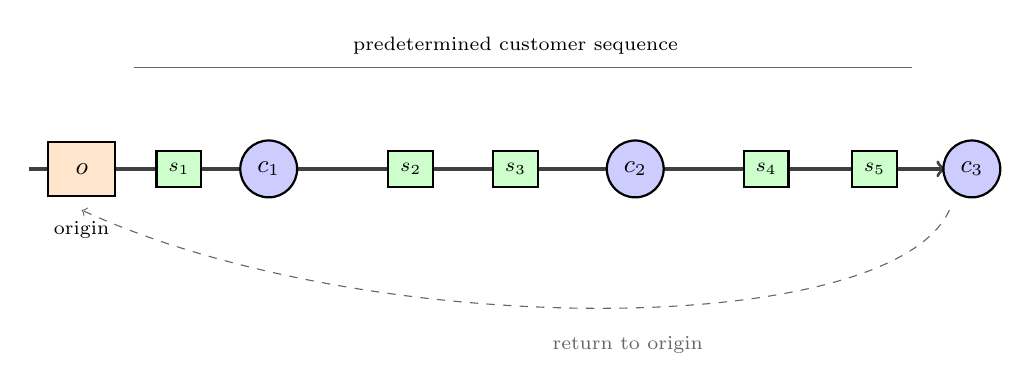
\begin{tikzpicture}[scale=0.95]

% ===================== main route =====================
\draw[very thick,->,color=black!75] (0,0) -- (12.25,0);
% \node at (17.05,0) {\scriptsize route direction};

% ===================== aligned guide lines =====================
\draw[thin,color=black!60] (1.4,1.35) -- (11.8,1.35);
\node at (6.5,1.65) {\scriptsize predetermined customer sequence};

% \draw[thin,color=black!60] (2.4,-1.35) -- (13.8,-1.35);
% \node at (8.1,-1.68) {\scriptsize predetermined customer sequence};

% \node at (8.1,2.25) {\scriptsize known distances and travel times between consecutive locations};

% ===================== origin =====================
\draw[thick,fill=orange!20] (0.25,-0.36) rectangle (1.15,0.36);
\node at (0.70,0) {\small $o$};
\node at (0.70,-0.82) {\scriptsize origin};

% % ===================== destination =====================
% \draw[thick,fill=orange!20] (14.85,-0.36) rectangle (15.75,0.36);
% \node at (15.30,0) {\small $d$};
% \node at (15.30,-0.82) {\scriptsize destination};

% ===================== customers (bigger) =====================
\draw[thick,fill=blue!20] (3.2,0) circle (0.38);
\node at (3.2,0) {\small $c_1$};

\draw[thick,fill=blue!20] (8.1,0) circle (0.38);
\node at (8.1,0) {\small $c_2$};

\draw[thick,fill=blue!20] (12.6,0) circle (0.38);
\node at (12.6,0) {\small $c_3$};

% ===================== charging stations =====================
% between origin and c1
\draw[thick,fill=green!20] (1.70,-0.24) rectangle (2.30,0.24);
\node at (2.00,0) {\scriptsize $s_1$};

% between c1 and c2
\draw[thick,fill=green!20] (4.80,-0.24) rectangle (5.40,0.24);
\node at (5.10,0) {\scriptsize $s_2$};

\draw[thick,fill=green!20] (6.20,-0.24) rectangle (6.80,0.24);
\node at (6.50,0) {\scriptsize $s_3$};

% between c2 and c3
\draw[thick,fill=green!20] (9.55,-0.24) rectangle (10.15,0.24);
\node at (9.85,0) {\scriptsize $s_4$};

\draw[thick,fill=green!20] (11.00,-0.24) rectangle (11.60,0.24);
\node at (11.30,0) {\scriptsize $s_5$};

% % between c3 and d
% \draw[thick,fill=green!20] (13.45,-0.24) rectangle (14.05,0.24);
% \node at (13.75,0) {\scriptsize $s_6$};

% % ===================== distance labels =====================
% \node[color=black!70] at (1.95,0.45) {\scriptsize $d_{o,1}$};
% \node[color=black!70] at (4.15,0.45) {\scriptsize $d_{1,2}$};
% \node[color=black!70] at (7.25,0.45) {\scriptsize $d_{2,3}$};
% \node[color=black!70] at (10.95,0.45) {\scriptsize $d_{3,4}$};
% \node[color=black!70] at (13.95,0.45) {\scriptsize $d_{4,d}$};

% ===================== dashed return arrow =====================
\draw[dashed,->,color=black!60] (12.30,-0.55) .. controls (11.5,-2.3) and (4.5,-2.3) .. (0.70,-0.55);
\node[color=black!60] at (8.0,-2.35) {\scriptsize return to origin};

\end{tikzpicture}
\caption{Illustrative route structure for the EVTDSP. The truck travels through a predetermined sequence of customers $(c_1,c_2,c_3)$ with charging stations $(s_1,s_2,s_3)$ available along the route.}
\label{fig:evtdsp_route}
\end{figure}


The route consists of a predetermined sequence of customer locations. Service at each customer requires a fixed duration and cannot be interrupted. Distances and travel times between consecutive locations are assumed known and deterministic. Energy consumption is assumed to be proportional to distance traveled and independent of cargo load. The BET is equipped with a battery of fixed capacity, measured in kilowatt-hours (kWh), and consumes energy at a constant rate proportional to distance traveled. The vehicle may recharge at CSs located at regular intervals along the route. All CSs are assumed to be homogeneous and provide energy at a fixed power level, implying a linear relationship between charging time and energy gained. Charging can be performed either fully or partially, and multiple charging stops are permitted throughout the route. However, recharging is not allowed during customer service.

The driver is subject to EU HoS regulations, which define allowable driving and working durations, as well as mandatory break and rest periods. Driving time includes only the operation of the vehicle between locations, while working time encompasses both driving and service time at customers. A break is a short pause  lasting (at least) 45 minutes, required after a maximum of 4.5 hours of driving. A daily rest is a longer, uninterrupted period, lasting at least 11 hours, and is required after a maximum of 9 hours of driving or 13 hours of total working time. An example of a valid HoS-compliant schedule is shown in Figure~\ref{fig:driver_schedule}. The regulation allows limited flexibility, such as the use of split rests or reduced rest durations under certain conditions. EU regulation allows certain flexibilities, including split breaks (e.g., 15+30 minutes) and reduced or split daily rests. For modeling clarity, the base formulation considers standard 45-minute breaks and full 11-hour daily rests. %These extensions can be incorporated by introducing additional rest arc types within the labeling framework, but are not required for the core analysis.

\begin{figure}[htbp!]
\centering
\resizebox{\textwidth}{!}{%
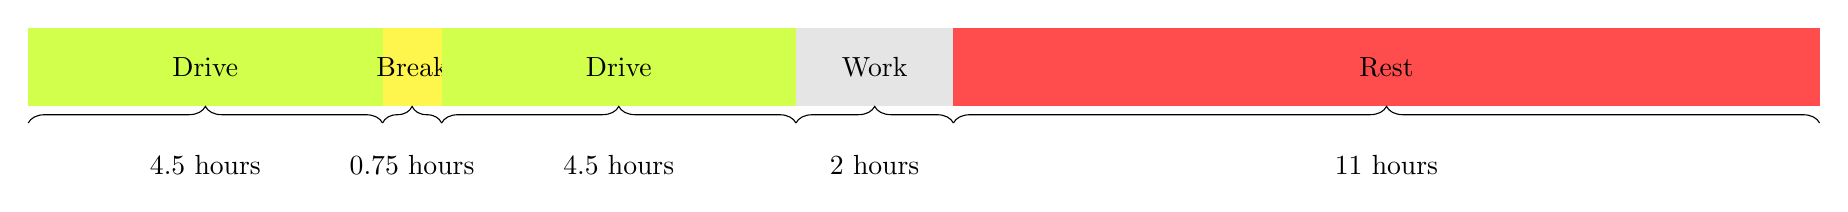
\begin{tikzpicture}
% Time blocks
\def\y{0}
\def\h{1}

\fill[fill=lime!70] (0,\y) rectangle (4.5,\y+\h);
\node at (2.25,\y+0.5) {Drive};

\fill[fill=yellow!70] (4.5,\y) rectangle (5.25,\y+\h);
\node at (4.875,\y+0.5) {Break};

\fill[fill=lime!70] (5.25,\y) rectangle (9.75,\y+\h);
\node at (7.5,\y+0.5) {Drive};

\fill[fill=gray!20] (9.75,\y) rectangle (11.75,\y+\h);
\node at (10.75,\y+0.5) {Work};

\fill[fill=red!70] (11.75,\y) rectangle (22.75,\y+\h);
\node at (17.25,\y+0.5) {Rest};

\draw[decorate,decoration={brace,amplitude=6pt},yshift=-6pt] (0,\y) -- (4.5,\y)
  node[midway,below=8pt] {4.5 hours};
\draw[decorate,decoration={brace,amplitude=6pt},yshift=-6pt] (4.5,\y) -- (5.25,\y)
  node[midway,below=8pt] {0.75 hours};
\draw[decorate,decoration={brace,amplitude=6pt},yshift=-6pt] (5.25,\y) -- (9.75,\y)
  node[midway,below=8pt] {4.5 hours};
\draw[decorate,decoration={brace,amplitude=6pt},yshift=-6pt] (9.75,\y) -- (11.75,\y)
  node[midway,below=8pt] {2 hours};
\draw[decorate,decoration={brace,amplitude=6pt},yshift=-6pt] (11.75,\y) -- (22.75,\y)
  node[midway,below=8pt] {11 hours};
\end{tikzpicture}%
}
\caption{Example of a schedule of a fully rested driver in accordance with EU HoS regulation.}
\label{fig:driver_schedule}
\end{figure}

Breaks and daily rests cannot be scheduled during customer service but may be taken at customer locations, charging stations, or intermediate points along the route. Charging and service activities are mutually exclusive, whereas charging may overlap with a break or rest if regulatory and physical constraints permit. At each feasible stopping location, decisions concern whether to initiate a break or rest and whether to recharge the battery, including the amount of energy added when charging is selected. Total route duration consists of driving time, service time, charging time, legally required interruptions. Feasible schedules therefore require consistent coordination of driver-state variables, battery energy levels, and temporal constraints across multiple days.
%

\section{ SPPRC Framework} %(Parameter-Free) SPPRC framework %Modelling approach

% \red{change structure again!}
% {
% \color{red}
% \begin{itemize}
%     \item start with the network from goel irnich (not extended with charging, very short description
%     \item THEN show our extension with charging (stations)
%     \item network and labeling algorithm should be presented together, as they are integrated (unfortunately)
% \end{itemize}
% }

The EVTDSP can be formulated as a shortest path problem with resource constraints (SPPRC) for constructing a feasible and time-efficient schedule along the prescribed route. The central challenge is therefore the joint scheduling of driving, service, charging, breaks, and daily rests under interacting HoS and battery constraints. Our modeling approach builds on the parameter-free network and labeling framework of \citet{goel2017exact}. In their setting, each travel arc between two consecutive customers is replaced by an activity subnetwork that explicitly represents the feasible sequencing of driver activities through resource extension functions (REFs). Starting from an auxiliary network in which activity durations are parameterized, Goel and Irnich show how this representation can be transformed into a parameter-free network, so that the duration of each elementary activity is determined directly from the current resource state and the associated feasibility conditions. This construction makes the resulting SPPRC amenable to an efficient labeling algorithm with strong dominance rules.

We extend this structure to the battery-electric setting by inserting charging stations as additional physical nodes on the fixed route. Each travel segment between two mandatory locations is therefore decomposed into one or more subsegments, each of which inherits the same activity structure as in Goel and Irnich. At a charging-station node, the schedule may either initiate a charging activity or pass through without charging. As a result, the extended network represents not only legally feasible sequences of driving, service, breaks, and rests, but also the choice of whether, where, and for how long to recharge between consecutive customers. Within this SPPRC framework, we consider two charging strategies. We first present a full-recharge strategy, in which each charging stop restores the battery to full capacity. We then generalize this model to a partial-recharge strategy, in which charging amounts are decision variables and the full-recharge case is recovered as a special case.


\subsection{Parameter-free network structure}
We now describe the activity network on which labels are propagated. The construction follows the parameter-free framework of \citet{goel2017exact} and extends it to accommodate charging-station visits. For a travel leg from a physical node \(n\) to the next physical node \(m\), the direct arc \((n,m)\) is replaced by a small activity subnetwork with two intermediate states, denoted by \(\tilde n_{nm}^{\mathrm{fit}}\) and \(\tilde n_{nm}^{\mathrm{dull}}\). The \emph{fit} state represents a situation in which the driver is able to continue driving, or has already completed the break or rest required before the next activity. The \emph{dull} state represents a situation in which the driver must take a break or rest before continuing. Arcs between these states correspond to elementary driver activities, namely starting a leg, driving, taking a break, taking a daily rest, and visiting the next physical node.

To model battery-electric operation, we insert charging stations as additional physical nodes along the fixed route. Hence, a leg between two mandatory locations may be decomposed into several consecutive sublegs, for example \((n,\mathrm{cs})\) and \((\mathrm{cs},m)\), each equipped with its own fit and dull states. At a charging-station node, the schedule may either initiate a charging activity or continue without charging. The former is represented by a visit arc at the charging station, whereas the latter is represented by pass-by arcs that preserve path continuity while bypassing the charging decision. In this way, the extended network captures both legally feasible activity sequences and the operational choice of whether to stop, recharge, and resume travel, or instead continue directly to the next segment.

The resulting network contains five classes of arcs: start arcs, driving arcs, break arcs, rest arcs, and visit arcs, together with pass-by arcs that allow a charging station to be traversed without stopping. A key feature of this representation is that a driving arc is not assigned a fixed duration in advance. Instead, its extension length \(\Delta\) is computed dynamically as the largest admissible driving time consistent with the current resource state. \(
\Delta
\)
is the minimum of (i) the remaining travel time to the next physical node, (ii) the remaining driving time until a mandatory break or daily rest, and (iii) the remaining daily working time before a mandatory rest must begin. In the electric-truck setting, the same principle is retained, but the resulting path must additionally remain energy-feasible. Consequently, each driving extension terminates either at the next physical node or at the point where HoS or energy considerations require a new decision. Figure~\ref{fig:subnetwork_cs} illustrates the resulting subnetwork for a route segment from customer \(n\) to customer \(m\) with an intermediate charging station.

\begin{figure}[!h]
\centering
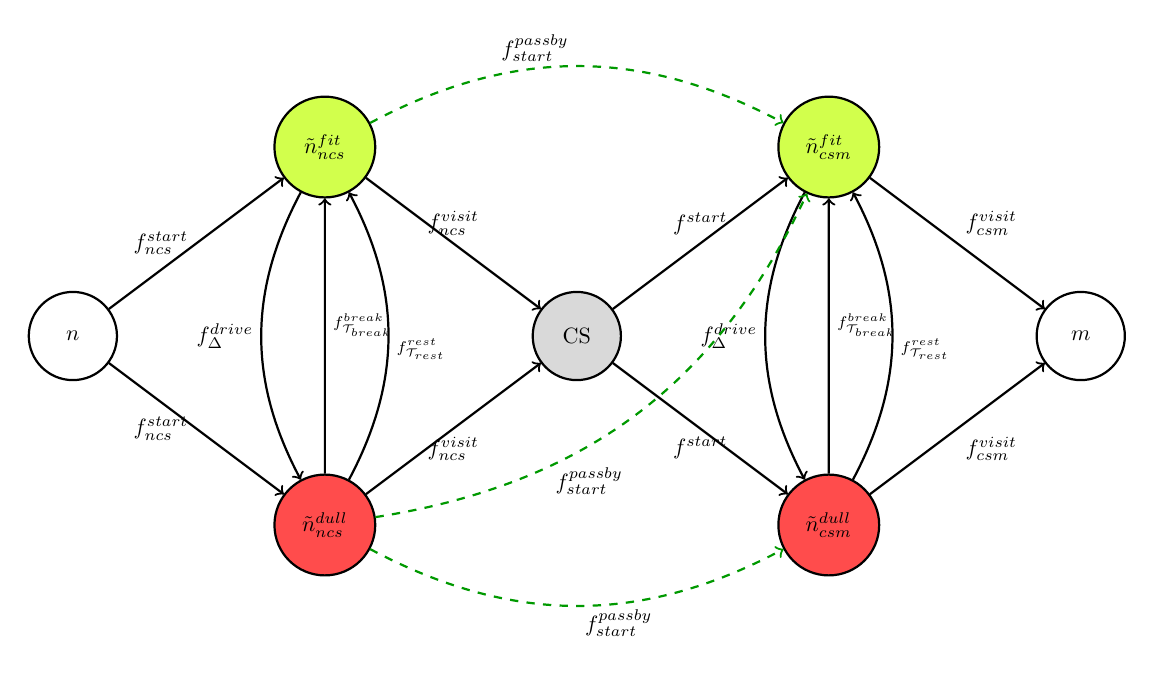
\begin{tikzpicture}[scale=0.8, transform shape, ->, thick, auto]
% Node styles
\tikzstyle{main} = [circle, draw=black, minimum size=1.4cm, inner sep=0pt]
\tikzstyle{fit}  = [circle, draw=black, fill=lime!70, minimum size=1.6cm, inner sep=0pt]
\tikzstyle{dull} = [circle, draw=black, fill=red!70, minimum size=1.6cm, inner sep=0pt]
\tikzstyle{cs}   = [circle, draw=black, fill=gray!30, minimum size=1.4cm, inner sep=0pt]

% Nodes
\node[main] (n) at (0,0) {$n$};
\node[fit]  (fitL) at (4, 3) {$\tilde{n}^{\text{fit}}_{ncs}$};
\node[dull] (dullL) at (4, -3) {$\tilde{n}^{\text{dull}}_{ncs}$};
\node[cs]   (cs) at (8, 0) {CS};
\node[fit]  (fitR) at (12, 3) {$\tilde{n}^{\text{fit}}_{csm}$};
\node[dull] (dullR) at (12, -3) {$\tilde{n}^{\text{dull}}_{csm}$};
\node[main] (m) at (16,0) {$m$};

% From n to left states
\path (n) edge node[left] {$f^{\text{start}}_{ncs}$} (fitL);
\path (n) edge node[left] {$f^{\text{start}}_{ncs}$} (dullL);

% Transitions between fit/dull (left side)
\path[bend right=28] (fitL) edge node[left] {$f^{\text{drive}}_{\Delta}$} (dullL);
\path (dullL) edge node[right, yshift=5pt] {\scriptsize $f^{\text{break}}_{\mathcal{T}_{\text{break}}}$} (fitL);
\path[bend right=28] (dullL) edge node[right, yshift=-6pt] {\scriptsize $f^{\text{rest}}_{\mathcal{T}_{\text{rest}}}$} (fitL);

% To CS
\path (fitL) edge node[above] {$f^{\text{visit}}_{ncs}$} (cs);
\path (dullL) edge node[below] {$f^{\text{visit}}_{ncs}$} (cs);

% From CS to right states
\path (cs) edge node[above] {$f^{\text{start}}$} (fitR);
\path (cs) edge node[below] {$f^{\text{start}}$} (dullR);

% Transitions between fit/dull (right side)
\path[bend right=28] (fitR) edge node[left] {$f^{\text{drive}}_{\Delta}$} (dullR);
\path (dullR) edge node[right, yshift=5pt] {\scriptsize $f^{\text{break}}_{\mathcal{T}_{\text{break}}}$} (fitR);
\path[bend right=28] (dullR) edge node[right, yshift=-6pt] {\scriptsize $f^{\text{rest}}_{\mathcal{T}_{\text{rest}}}$} (fitR);

% From right states to m
\path (fitR) edge node[above right] {$f^{\text{visit}}_{csm}$}  (m);
\path (dullR) edge node[below right] {$f^{\text{visit}}_{csm}$} (m);

% Passing-by arcs
\path[->, dashed, thick, green!60!black, bend left=28]
  (fitL) edge node[left, yshift=8pt] {\textcolor{black}{$f^{\text{passby}}_{\text{start}}$}} (fitR);
\path[->, dashed, thick, green!60!black, bend right=28]
  (dullL) edge node[right, xshift=-40pt, yshift=-30pt] {\textcolor{black}{$f^{\text{passby}}_{\text{start}}$}} (fitR);
\path[->, dashed, thick, green!60!black, bend right=28]
  (dullL) edge node[right, yshift=-8pt] {\textcolor{black}{$f^{\text{passby}}_{\text{start}}$}} (dullR);
\end{tikzpicture}
\caption{Extended subnetwork with a charging station (CS) enabling transitions.}
\label{fig:subnetwork_cs}
\end{figure}


\begin{comment}
    

\subsection{Parameter-free network structure}


The EVTDSP defined above can be reformulated as a shortest path problem with resource constraints (SPPRC). Since the sequence of customer visits is fixed, the routing component is predetermined and the planning task reduces to constructing a feasible and time-efficient schedule along this ordered sequence. The core challenge lies not in selecting the order of visits, but in determining the timing and synchronization of driving, service, charging, breaks, and daily rest periods under interdependent regulatory and energy constraints.


To model feasible activity sequences through the network without discretizing time, we adopt the parameter-free network representation introduced by \citet{goel2017exact} and extend it to incorporate battery-electric operation.

\paragraph{Node structure}
Let the route consist of an ordered sequence of nodes, which can represent customers as well as charging stations.
Between each consecutive pair of physical nodes on the fixed route, the network containss auxiliary intermediate nodes denoted $\tilde{n}^{\text{fit}}$ and $\tilde{n}^{\text{dull}}$.
\red{Is this interpretation actually correct? I would rephrase it...}
The \emph{fit} node represents a state in which a new activity may start (e.g., driving or charging), whereas the \emph{dull} node captures the continuation or termination of an ongoing activity, for instance completing a break or finishing a rest. Arcs between these nodes correspond to elementary operations: driving, breaks, rests, customer service, and charging.

Figure~\ref{fig:subnetwork_cs} illustrates this structure for a segment connecting a customer node $n$ to a customer node $m$ via an intermediate charging station (CS). 

    
\begin{figure}
\FIGURE
{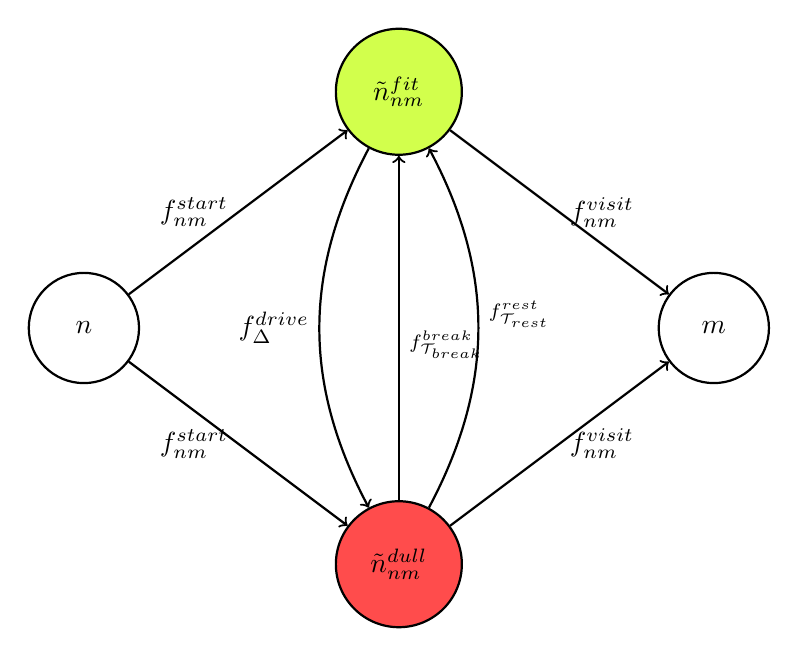
\begin{tikzpicture}[->, thick, auto]
% Node styles
\tikzstyle{main} = [circle, draw=black, minimum size=1.4cm, inner sep=0pt]
\tikzstyle{fit} = [circle, draw=black, fill=lime!70, minimum size=1.6cm, inner sep=0pt]
\tikzstyle{dull} = [circle, draw=black, fill=red!70, minimum size=1.6cm, inner sep=0pt]
% Nodes
\node[main] (n) at (0,0) {$n$};
\node[main] (m) at (8,0) {$m$};
\node[fit] (fit) at (4,3) {$\tilde{n}_{nm}^{\text{fit}}$};
\node[dull] (dull) at (4,-3) {$\tilde{n}_{nm}^{\text{dull}}$};
% Arrows from n to intermediates
\path (n) edge node[left] {$f^{\text{start}}_{nm}$} (fit);
\path (n) edge node[left] {$f^{\text{start}}_{nm}$} (dull);
% Arrows from intermediates to m
\path (fit) edge node[right] {$f^{\text{visit}}_{nm}$} (m);
\path (dull) edge node[right] {$f^{\text{visit}}_{nm}$} (m);
% Curved arrows between intermediates
\path[bend right=28] (dull) edge node[right, yshift=5pt] {\scriptsize $f^{\text{rest}}_{\mathcal{T}_{\text{rest}}}$} (fit);
\path (dull) edge node[right, yshift=-6pt] {\scriptsize $f^{\text{break}}_{\mathcal{T}_{\text{break}}}$} (fit);
\path[bend right=28] (fit) edge node[left] {$f^{\text{drive}}_{\Delta}$} (dull);
\end{tikzpicture}}
{Subnetwork \(G''_{nm}\) of the parameter-free network \(G''\). \label{fig:subnetwork_nm}}
{Text of the notes.}
\end{figure}


\paragraph{Arc structure}
Directed arcs correspond to elementary activities:
\begin{itemize}
    \item start arcs initiating movement,
    \item driving arcs $f^{\text{drive}}_{\Delta}$,
    \item break and rest arcs,
    \item visit arcs representing customer service or charging activity,
    \item pass-by arcs allowing continuation without charging.
\end{itemize}
This structure compactly encodes all admissible sequences of driving, resting, servicing, and charging between consecutive customers.


\paragraph{Resources}
Feasibility is enforced through a multidimensional resource vector that evolves along each arc. The resources track:
\begin{enumerate}
    \item total elapsed time,
    \item continuous and cumulative driving and working times under EU HoS regulations,
    \item battery energy consumption and state of charge.
\end{enumerate}

\paragraph{Driving extension length}
The duration $\Delta$ of a driving arc is determined dynamically to ensure regulatory feasibility. Following \citet{goel2017exact}, $\Delta$ is defined as the largest admissible continuous driving time such that none of the following constraints is violated:
\begin{itemize}
    \item remaining travel time to the next physical node,
    \item maximum continuous driving time before a break,
    \item maximum cumulative driving time before a daily rest,
    \item maximum allowable working time within the current day.
\end{itemize}
Thus, $\Delta$ is chosen as the minimum of the remaining allowable durations implied by these limits. Each driving arc therefore terminates either upon reaching the next node or when a regulatory constraint becomes binding.

\end{comment}



\subsection{Labeling algorithm}

We solve the resulting SPPRC by a labeling algorithm on the parameter-free activity network. Each label represents a partial path together with the associated driver and vehicle resource state, and feasible schedules are constructed incrementally through label extension and resource propagation.

The algorithm starts from a single initial label at the depot, corresponding to a fully rested and fully charged vehicle-driver state. At each iteration, an unprocessed label is selected and extended along all outgoing arcs that are feasible with respect to the current resource state. Each extension generates a new label whose temporal, regulatory, and energy-related resources are updated according to the REF of the traversed arc. Labels that violate HoS, or battery-feasibility conditions are discarded immediately. Whenever several labels reach the same network node, dominance rules are applied to eliminate labels that cannot lead to a better feasible completion than another label at that node. In this way, the algorithm explores only nondominated partial schedules. A label is complete when it reaches the terminal node after all mandatory visits have been performed in the prescribed order.

We first present the full-recharge strategy and then extend this model to partial recharging, in which charging amounts become decision variables. The partial-recharge formulation generalizes the full-recharge case, which is recovered when each charging action restores the battery to full capacity. The remainder of this subsection specifies the label definition, the resource extension functions, and the associated feasibility and dominance rules.

% Algorithm~\ref{alg:labeling-algorithm} summarizes the overall solution procedure.

% We solve the resulting SPPRC by a labeling algorithm on the parameter-free activity network. A label represents a partial path from the origin to a network node together with the corresponding resource state of the driver and vehicle. Thus, the labeling procedure constructs schedules incrementally by extending labels along feasible outgoing arcs and updating their resources through the associated resource extension functions.

% The algorithm starts from a single initial label at the depot, corresponding to a fully rested and fully charged vehicle-driver state. At each iteration, an unprocessed label is selected and extended along all outgoing arcs that are feasible with respect to the current resource state. Each extension generates a new label whose time, HoS counters, and energy-related resources are updated according to the REF of the traversed arc. Labels that violate time-window, HoS, or battery-feasibility conditions are discarded immediately. Whenever several labels reach the same network node, dominance rules are applied to eliminate labels that cannot lead to a better feasible completion than another label at that node. In this way, the algorithm explores only nondominated partial schedules. A label is complete when it reaches the terminal node after all mandatory visits have been performed in the prescribed order. 

% The remainder of this section specifies the components of the labeling algorithm. We first define the label structure and the associated resource vector. We then present the resource extension functions used to propagate labels through the network, followed by the feasibility and dominance rules that ensure correctness and computational tractability. Algorithm~\ref{alg:labeling-algorithm} summarizes the overall solution procedure.

\begin{comment}
    
\begin{algorithm}
\caption{Labeling Algorithm}\label{alg:labeling-algorithm}
\vskip6pt
\begin{algorithmic}
\Require Network graph \( G = (N, A) \)
\Ensure Set of processed labels \( P \)

\Statex \textit{// Initialize the empty set of processed labels}
\State \( P \gets \emptyset \)
\Statex \textit{// Initialize with label for the start node}
\State \( U \gets \{(s)\} \)
\While{\( U \neq \emptyset \)}
    \State \( U \gets \text{timeAscendingSort}(U) \)
    \State \( L \gets U[0] \)
    \ForAll{arc \( A \in (i, j) \)}
        \State Create new label \( L' \gets \text{copy of } L \)
        \State Extend \( L' \) using appropriate REF
        \If{\( L' \) is resource feasible}
            \State Add \( L' \) to \( U \)
            \If{\( L' \) has visited all cities}
                \State Mark \( L' \) as processed
                \State Add \( L' \) to \( P \)
            \EndIf
        \EndIf
    \EndFor
    \State Mark \( L \) as processed
    \State Add \( L \) to \( P \)

    \Statex \textit{// Dominance step}
    \State Apply dominance function to \( U \)
    \ForAll{element \( e \) dominated in \( U \)}
        \State Mark \( e \) as processed
        \State Add \( e \) to \( P \)
        \State Remove \( e \) from \( U \)
    \EndFor
\EndWhile
\State \Return \( P \)
\end{algorithmic}
\end{algorithm}

The labeling algorithm is well-suited for our parameter-free network structure. It efficiently captures the temporal evolution of driver and vehicle state, avoids redundant extensions via dominance pruning, and supports flexible break-recharge synchronization through modular REFs.

\end{comment}


\subsubsection{Label definition}

A label \(l\) represents a partial path from the origin to a network node together with the temporal, regulatory, and energy state of the driver--vehicle system required to continue that partial schedule.

All labels, irrespective of the charging strategy, maintain the same Hours-of-Service resources and the same interpretation of the temporal state. The difference between the two strategies lies in how the temporal and energy-related components are represented: scalar-valued under full recharge and interval-valued under partial recharge. The resource \(l_{\text{time}}\) records the total time elapsed since departure. The resource \(l_{\text{timeToNext}}\) denotes the remaining driving time to the next physical node and is particularly important for modeling traversal between intermediate fit and dull states; it becomes zero when a customer or charging station has been reached. The counters \(l_{\text{drive|R}}\) and \(l_{\text{drive|B}}\) track accumulated driving time since the last daily rest and since the last break, respectively, while \(l_{\text{elapsed|R}}\) and \(l_{\text{elapsed|B}}\) record the corresponding elapsed working time. 

% The variables \(l_{\text{latest|R}}\) and \(l_{\text{latest|B}}\) store the latest feasible completion times of the next rest and break implied by downstream time windows. 

In contrast to \citet{goel2017exact}, we explicitly retain the break-specific counters \(l_{\text{drive|B}}\), \(l_{\text{elapsed|B}}\). In our setting these resources can become binding and are necessary to preserve exact compliance with the EU break rules. Table~\ref{tab:resource_windows} summarizes the corresponding feasibility windows. Under the full-recharge strategy, each charging stop restores the battery to full capacity. The energy state can therefore be represented by a single scalar resource \(l_{\text{reqEC}}\), which measures the energy requirement accumulated since the last recharge. Equivalently, the state of charge after any partial path is uniquely determined by \(B-l_{\text{reqEC}}\), where \(B\) denotes the battery capacity. A full-recharge label is thus defined as
\[
\begin{aligned}
l = (&l_{\text{time}},\, l_{\text{timeToNext}},\, l_{\text{drive|R}},\\
     &l_{\text{drive|B}},\, l_{\text{elapsed|R}},\, l_{\text{elapsed|B}},\\
     &l_{\text{reqEC}})
\end{aligned}
\]

% \[
% \begin{aligned}
% l = (&l_{\text{time}},\, l_{\text{timeToNext}},\, l_{\text{drive|R}},\\
%      &l_{\text{drive|B}},\, l_{\text{elapsed|R}},\, l_{\text{elapsed|B}},\\
%      &l_{\text{latest|R}},\, l_{\text{latest|B}},\, l_{\text{reqEC}})
% \end{aligned}
% \]

The resource \(l_{\text{reqEC}}\) is bounded by \(0 \leq l_{\text{reqEC}} \leq B\). Its design is inspired by \citet{desaulniers2016exact}, but we retain an energy-based rather than time-based representation in order to preserve flexibility across different battery capacities, charging powers, and energy-consumption rates.

When partial recharging is allowed, the amount charged at a station becomes a decision variable. As a consequence, labels arriving at the same node may represent a continuum of feasible time--energy trade-offs. To capture these trade-offs compactly, the time and energy components of the label are represented by intervals. Specifically, we maintain a time interval \([l_{\text{time}}^{\min},l_{\text{time}}^{\max}]\), an energy-deficit interval \([l_{\text{reqEC}}^{\min},l_{\text{reqEC}}^{\max}]\), and a state-of-charge interval \([l_{\text{SOC}}^{\min},l_{\text{SOC}}^{\max}]\). The HoS-related counters are propagated exactly as in the full-recharge strategy, since regulatory feasibility depends on the temporal evolution of activities rather than on the precise state of charge. A partial-recharge label is therefore written as

% \[
% \begin{aligned}
% l = (&l_{\text{time}}^{\min},\, l_{\text{time}}^{\max},\, l_{\text{timeToNext}}, l_{\text{drive|R}},\, l_{\text{drive|B}},\\
%      &l_{\text{elapsed|R}},\, l_{\text{elapsed|B}},
%      l_{\text{latest|R}},\, l_{\text{latest|B}},\\
%      &l_{\text{reqEC}}^{\min},\, l_{\text{reqEC}}^{\max},
%      l_{\text{SOC}}^{\min},\, l_{\text{SOC}}^{\max})
% \end{aligned}
% \]

\[
\begin{aligned}
l = (&l_{\text{time}}^{\min},\, l_{\text{time}}^{\max},\, l_{\text{timeToNext}}, l_{\text{drive|R}},\, l_{\text{drive|B}},\\
     &l_{\text{elapsed|R}},\, l_{\text{elapsed|B}}, \\ 
     &l_{\text{reqEC}}^{\min},\, l_{\text{reqEC}}^{\max},
     l_{\text{SOC}}^{\min},\, l_{\text{SOC}}^{\max})
\end{aligned}
\]
The partial-recharge model generalizes the full-recharge strategy: the latter is recovered when the energy-related intervals collapse to singletons after each charging operation. Feasibility of each label extension is enforced by requiring all resource components to remain within their prescribed bounds. Under partial recharge, the feasibility bounds in Table~\ref{tab:resource_windows} apply componentwise to the corresponding interval endpoints.

\begin{table}[!htbp]
\centering
\caption{Label resources with corresponding resource windows.}
\label{tab:resource_windows}
\begin{tabular}{@{}lll@{}}
\toprule
\textbf{Resource} & \textbf{Description} & \textbf{Feasibility Window} \\
\midrule
$ \text{time} $ & Total time elapsed since start & $ [t^{\min}_n, t^{\max}_n] \cap [0, T_{\text{horizon}}] $ \\
$ \text{timeToNext} $ & Remaining driving time to next node & $ [0, t_{nm}] $ \\
$ \text{drive|R} $ & Driving time since last rest & $ [0, t_{\text{drive}|R}] $ \\
$ \text{drive|B} $ & Driving time since last break & $ [0, t_{\text{drive}|B}] $ \\
$ \text{elapsed|R} $ & Elapsed time since last rest & $ [0, t_{\text{elapsed}|R}] $ \\
$ \text{elapsed|B} $ & Elapsed time since last break & $ [0, t_{\text{elapsed}|B}] $ \\
% $ \text{latest|R} $ & Latest time rest must end & $ [0, \infty) $ \\
% $ \text{latest|B} $ & Latest time break must end & $ [0, \infty) $ \\
$ \text{reqEC} $ & Required energy since last recharge & $ [0, B] $ \\
\bottomrule
\end{tabular}
\end{table}




\begin{comment}
  
A label $l$ corresponds to a partial path from the origin to a given network node and is defined by a multidimensional resource vector capturing the temporal, regulatory, and energy state of the vehicle and driver.

To accommodate partial recharging, the time and energy components are represented as intervals. 

A label at a network node is defined as the tuple \[
l = \big(
l^{\min}_{t},\, l^{\max}_{t},\,
l^{R}_{d},\, l^{B}_{d},\,
l^{R}_{e},\, l^{B}_{e},\,
l^{SOC}
\big),
\]
where:
\begin{itemize}
    \item $[l^{\min}_{t}, l^{\max}_{t}]$ is the interval of feasible arrival times,
    \item $l^{R}_{d}$ is the accumulated driving time since the last daily rest,
    \item $l^{B}_{d}$ is the accumulated driving time since the last break,
    \item $l^{R}_{e}$ is the elapsed working time since the last daily rest,
    \item $l^{B}_{e}$ is the elapsed working time since the last break,
    \item $[l^{SOC}$ \red{to do together with mostafa}
\end{itemize}

A label therefore contains:

\begin{itemize}
    \item a time interval $[l^{\min}_{\text{time}}, l^{\max}_{\text{time}}]$,
    \item continuous and cumulative driving and working counters under EU HoS rules,
    \item an energy-deficit interval $[l^{\min}_{\text{reqEC}}, l^{\max}_{\text{reqEC}}]$,
    \item the corresponding state-of-charge bounds.
\end{itemize}


Under partial recharge, the time and energy components of the label become interval-valued. In particular, we maintain:
(i) a time interval \([l_{\text{time}}^{\min},\, l_{\text{time}}^{\max}]\),
(ii) an energy-deficit interval \([l_{\text{reqEC}}^{\min},\, l_{\text{reqEC}}^{\max}]\), and
(iii) a state-of-charge interval \([l_{\text{SOC}}^{\min},\, l_{\text{SOC}}^{\max}]\).
All HoS-related counters (\(l_{\text{drive|R}}, l_{\text{drive|B}}, l_{\text{elapsed|R}}, l_{\text{elapsed|B}}, l_{\text{latest|R}}, l_{\text{latest|B}}\)) are propagated as in the full-recharge strategy, since the HoS rules depend on the temporal evolution of activities and not on the precise SoC level.

The full-recharge model is obtained as a special case where the energy interval collapses to a singleton after each charging operation.




The resource \( \text{time} \) represents the total time elapsed since the beginning of the route and must respect both the global horizon and customer-specific time windows. \( \text{timeToNext} \) indicates the remaining driving time to the next node and is particularly important for modeling traversal between intermediate fit and dull nodes. A value of zero for this resource signifies that a customer or charging station has been reached.

The resources \( \text{drive|R} \) and \( \text{drive|B} \) track the accumulated driving time since the last rest and break, respectively. Similarly, \( \text{elapsed|R} \) and \( \text{elapsed|B} \) capture the total elapsed time (including driving and working) since the last rest or break. These four values collectively enforce the rolling and daily legal constraints imposed by EU HoS rules. The variables \( \text{latest|R} \) and \( \text{latest|B} \) represent soft deadlines for completing the next rest or break in order to ensure feasibility with downstream customer time windows.

Feasibility of each label extension is enforced by requiring that all components of the resource vector remain within predefined bounds. These bounds are specified in Table~\ref{tab:resource_windows}. For example, the resource \( \text{drive|R} \) is constrained to lie within the interval \([0, t_{\text{drive}|R}]\), reflecting the maximum allowable continuous driving time before a rest is mandatory.

A major extension introduced in our model is the resource \( \text{reqEC} \), which represents the energy requirement accrued since the last recharge. This resource is used to model battery depletion and is essential for ensuring that the truck recharges sufficiently before continuing to the next segment. The design of \( \text{reqEC} \) is inspired by the work of \citet{desaulniers2016exact}, though we deviate from their later time-based accounting to maintain flexibility across varying battery sizes, energy consumption rates, and charging powers. The upper bound of \( \text{reqEC} \) is equal to the battery capacity \( B \). Table~\ref{tab:resource_windows} provides a full description of each label resource and its corresponding feasibility window, ensuring legal and physical constraints are respected throughout the route.

\begin{table}
\TABLE
{Label resources with corresponding description and resource windows (adapted from Table 5.1).\label{tab:resource_windows}}
{\begin{tabular}{@{}lll@{}}
\hline\up
\textbf{Resource} & \textbf{Description} & \textbf{Feasibility Window} \\
\hline\up
$ \text{time} $ & Total time elapsed since start & $ [t^{\min}_n, t^{\max}_n] \cap [0, T_{\text{horizon}}] $ \\
$ \text{timeToNext} $ & Remaining driving time to next node & $ [0, t_{nm}] $ \\
$ \text{drive|R} $ & Driving time since last rest & $ [0, t_{\text{drive}|R}] $ \\
$ \text{drive|B} $ & Driving time since last break & $ [0, t_{\text{drive}|B}] $ \\
$ \text{elapsed|R} $ & Elapsed time since last rest & $ [0, t_{\text{elapsed}|R}] $ \\
$ \text{elapsed|B} $ & Elapsed time since last break & $ [0, t_{\text{elapsed}|B}] $ \\
$ \text{latest|R} $ & Latest time rest must end & $ [0, \infty) $ \\
$ \text{latest|B} $ & Latest time break must end & $ [0, \infty) $ \\
$ \text{reqEC} $ & Required energy since last recharge & $ [0, B] $ \down\\
\hline
\end{tabular}}
{Table Notes.}
\end{table}


\red{
To support EU HoS compliance more precisely, we reintroduce break-specific resource counters \( l_{\text{drive|B}} \), \( l_{\text{elapsed|B}} \), and \( l_{\text{latest|B}} \), which Goel and Irnich omitted under the assumption that they were non-binding. Our computational tests showed that omitting these counters can result in schedules that violate the 4.5-hour continuous driving limit or 6-hour working limit between breaks—prompting their reinstatement in our model.
}
\end{comment}

\subsubsection{Resource extension functions}

Each arc \(a\in A\) of the parameter-free network is associated with a resource extension function (REF)
\(
f_a:\mathcal{L}\rightarrow\mathcal{L},
\)
which maps a feasible label \(l\) at the tail node of \(a\) to a new label \(l'=f_a(l)\) at its head node. The REFs govern how the temporal, regulatory, and energy-related components of a label evolve when a partial schedule is extended by one elementary activity.

Under both charging strategies, five REFs are inherited from the parameter-free framework of \citet{goel2017exact}: \(f^{\text{start}}_{nm}\), \(f^{\text{drive}}_{\Delta}\), \(f^{\text{break}}_{\Delta}\), \(f^{\text{rest}}_{\Delta}\), and \(f^{\text{visit}}_{nm}\). The start REF initializes a new travel leg by setting the remaining travel time to the next physical node. The drive REF propagates time and HoS counters over a driving period of duration \(\Delta\). The break and rest REFs advance time and reset the corresponding regulatory counters. The visit REF models the service or stop activity at a physical node, including time-window alignment and the induced update of the latest feasible break and rest completion times.

As in \citet{goel2017exact}, the duration \(\Delta\) of a driving extension is determined endogenously from the current resource state. Specifically,
\[
\begin{aligned}
\Delta = \min\Bigl\{\, &
l_{\text{timeToNext}},\,
t_{R}^{\text{drive}} - l_{\text{drive},R},\,
t_{B}^{\text{drive}} - l_{\text{drive},B},\\
&
t^{\text{day}} - \bigl(l_{\text{elapsed},R} + t_{\text{rest}}\bigr)
\Bigr\}.
\end{aligned}
\]
Hence, a driving arc terminates either when the next physical node is reached or when a break, a rest, or the daily working-time limit becomes binding.

For the full-recharge strategy, charging at a station \(\mathrm{cs}\) is represented by an additional REF \(f^{\text{recharge}}_{\mathrm{cs}}\). This extension resets the accumulated energy requirement \(l_{\text{reqEC}}\) to zero and increases the elapsed time by the charging duration implied by the current energy deficit and the available charging power. When charging overlaps with a legally admissible break or rest, the corresponding HoS counters are updated consistently so that synchronization between charging and regulatory interruptions is captured directly in the label propagation. In addition, pass-by arcs are modeled through \(f^{\text{passby}}_{\text{start}}\), which allows a charging station to be traversed without stopping while preserving all resource values except the remaining travel time to the next physical node.

Under the partial-recharge strategy, the same network structure and the same common REFs are retained. The only difference is that the charging extension no longer restores the battery to full capacity. Instead, \(f^{\text{recharge}}_{\mathrm{cs}}\) propagates an interval of feasible time--energy outcomes, reflecting the fact that the charging amount is itself a decision variable. The full-recharge strategy is recovered as the special case in which this interval collapses to a singleton corresponding to a complete recharge.

Table~\ref{tab:ref_all} summarizes the resource updates for the common REFs together with the full-recharge charging and pass-by extensions. These updates form the computational core of the labeling algorithm; the partial-recharge variant preserves the same structure but replaces the scalar charging update by its interval-valued counterpart.


\begin{table}[!htbp]
\caption{Resource updates for the common REFs and the full-recharge charging extension.}
\label{tab:ref_all}
\centering
\small
\setlength{\tabcolsep}{2.5pt}
\renewcommand{\arraystretch}{1.15}
\resizebox{\linewidth}{!}{%
\begin{tabular}{@{}lccccccc@{}}
\toprule
\textbf{Resource} & \( f^{\text{start}}_{nm} \) & \( f^{\text{drive}}_{\Delta} \) & \( f^{\text{break}}_{\Delta} \) & \( f^{\text{rest}}_{\Delta} \) & \( f^{\text{visit}}_{nm} \) & \( f^{\text{recharge}}_{\text{cs}} \) & \( f^{\text{passby}}_{\text{start}} \) \\
\midrule
\( l'_{\text{time}} \) & --- & \( l_{\text{time}} + \Delta \) & \( l_{\text{time}} + t_{\text{break}} \) & \( l_{\text{time}} + t_{\text{rest}} \) & \( \max\{l_{\text{time}}, T^{\min}_m\} + s_m \) & \( \begin{cases}
l_{\text{time}} & l_{\text{elapsed|R}} = 0 \\
l_{\text{time}} + \max\left\{0, \frac{l_{\text{reqEC}}}{CP} - t_{\text{break}} \right\} & l_{\text{elapsed|B}} = 0 \\
l_{\text{time}} + \frac{l_{\text{reqEC}}}{CP} & \text{otherwise}
\end{cases} \) & --- \\
\( l'_{\text{timeToNext}} \) & \( t_{nm} \) & \( l_{\text{timeToNext}} - \Delta \) & --- & --- & --- & \( t_{\text{cs},m} \) & \( t_{\text{cs},m} \) \\
\( l'_{\text{drive|R}} \) & --- & \( l_{\text{drive|R}} + \Delta \) & --- & 0 & --- & --- & --- \\
\( l'_{\text{drive|B}} \) & --- & \( l_{\text{drive|B}} + \Delta \) & 0 & 0 & --- & --- & --- \\
\( l'_{\text{elapsed|R}} \) & --- & \( l_{\text{elapsed|R}} + \Delta \) & \( l_{\text{elapsed|R}} + t_{\text{break}} \) & 0 & \( \max\{l_{\text{elapsed|R}}, T^{\min}_m - l_{\text{latest|R}}\} + s_m \) & \( \begin{cases}
0 & l_{\text{elapsed|R}} = 0 \\
l_{\text{elapsed|R}} + \frac{l_{\text{reqEC}}}{CP} & \text{otherwise}
\end{cases} \) & --- \\
\( l'_{\text{elapsed|B}} \) & --- & \( l_{\text{elapsed|B}} + \Delta \) & 0 & 0 & \( \max\{l_{\text{elapsed|B}}, T^{\min}_m - l_{\text{latest|B}}\} + s_m \) & \( \begin{cases}
0 & l_{\text{elapsed|B}} = 0 \\
l_{\text{elapsed|B}} + \frac{l_{\text{reqEC}}}{CP} & \text{otherwise}
\end{cases} \) & --- \\
\( l'_{\text{reqEC}} \) & 0 & \( l_{\text{reqEC}} + \Delta \cdot \alpha \) & --- & --- & --- & 0 & --- \\
\bottomrule
\end{tabular}%
}
\end{table}

\begin{comment}
    
\subsubsection{Resource extension functions}
Each arc $a \in A$ of the parameter-free network is associated with a 
resource extension function (REF)
\[
f_a : \mathcal{L} \rightarrow \mathcal{L},
\]
which maps a feasible label $l$ at the tail node of $a$ to a new label
$l' = f_a(l)$ at its head node.


\red{Write much more efficient, define everything at once, only highlight afterwards what is new?}
In the original formulation, five core REFs govern label propagation across a parameter-free subnetwork: \( f^{\text{start}}_{nm} \), \( f^{\text{drive}}_{\Delta} \), \( f^{\text{break}}_{\Delta} \), \( f^{\text{rest}}_{\Delta} \), and \( f^{\text{visit}}_{nm} \). These functions define how the resource vector evolves based on the driver's actions. For example, \( f^{\text{start}}_{nm} \) initializes the driving segment between two customer nodes by setting the required travel time \( t_{nm} \) without incrementing the elapsed time. The REF \( f^{\text{drive}}_{\Delta} \) increases time, energy consumption, and accumulated driving counters over a continuous driving segment of length \( \Delta \). The break and rest REFs reset relevant counters, while \( f^{\text{visit}}_{nm} \) models customer service operations, accounting for service time and time window alignment. These operations and their impacts on resources are summarized in Table~\ref{tab:ref_all}.

To model Battery Electric Truck operations, we introduce an additional REF: \( f^{\text{recharge}}_{\text{cs}} \). This REF is used when visiting a charging station and updates the energy-related resource \( l_{\text{reqEC}} \). Charging duration is determined by the energy deficit divided by the available charging power \( CP \). If the charging time exceeds the legal break requirement (typically 45 minutes), it can also reset regulatory counters thereby satisfying both energy and HoS constraints simultaneously. The corresponding update logic is included in Table~\ref{tab:ref_all}.


In addition to modeling recharging, we extend the network with a mechanism to pass through charging stations without stopping. This is handled by a new REF: \( f^{\text{passby}}_{\text{start}} \), used when a label encounters a charging station node but has no need to recharge. This REF allows the label to bypass the charging activity while maintaining label continuity, updating only the remaining travel time \( t_{\text{cs},m} \) to the next node. All other resources remain unchanged, as shown in the final column of Table~\ref{tab:ref_all}.

The maximum extension duration \( \Delta \) for driving activities is dynamically computed to ensure regulatory compliance. It is defined in Equation~\ref{eq:delta}:

\begin{equation}\label{eq:delta}
\begin{aligned}
\Delta = \min \Bigl\{&
l_{\text{timeToNext}},\ 
t^{\text{drive}}_R - l_{\text{drive|R}},\\ 
t^{\text{drive}}_B - l_{\text{drive|B}},\
& t^{\text{day}} - (l_{\text{elapsed|R}} + t_{\text{rest}})
\Bigr\}
\end{aligned}
\end{equation}


This constraint ensures that label extensions remain within the bounds of continuous and cumulative driving regulations, as well as total daily working time.

A complete view of how these REFs manipulate resource states is presented in Table~\ref{tab:ref_all}, which consolidates the behavior of all REF types, including recharging and pass-by arcs. Together, these REFs constitute the computational core of the labeling algorithm, enabling the construction of feasible schedules that are both regulation-compliant and energy-efficient.

\end{comment}

\subsubsection{Feasibility and dominance}

After each resource extension, the resulting label must remain feasible. Feasibility is enforced with respect to two dimensions: time windows, Hours-of-Service requirements, and energy availability. Only labels that satisfy all three are retained for further extension.

Time feasibility requires that service at each customer node \(n\in N\) respect the corresponding time window \([t_n^{\min},t_n^{\max}]\), while the overall elapsed time remains within the planning horizon. Regulatory feasibility is enforced through the driving and elapsed-time counters \(l_{\text{drive|R}}\), \(l_{\text{drive|B}}\), \(l_{\text{elapsed|R}}\), and \(l_{\text{elapsed|B}}\), which must remain within their respective limits. In addition, the auxiliary resources \(l_{\text{latest|R}}\) and \(l_{\text{latest|B}}\) impose latest feasible completion times for the next rest and break implied by downstream time windows. These bounds ensure that a label is not only currently feasible, but can also be extended without violating future temporal requirements.

Energy feasibility is captured through the accumulated energy requirement since the last recharge. Under the full-recharge strategy, this is the scalar resource \(l_{\text{reqEC}}\), which must remain within \([0,B]\) and is reset to zero by a recharge extension. Under the partial-recharge strategy, the corresponding energy and state-of-charge intervals must remain feasible componentwise. Finally, the network structure itself imposes local feasibility conditions: traversals between fit and dull states are admissible only when the associated regulatory and energy requirements of the corresponding activity are satisfied.

To limit the number of labels carried forward, we apply dominance at each network node. Let \(l_1\) and \(l_2\) be two labels ending at the same node. Under the full-recharge strategy, \(l_1\) dominates \(l_2\) if
\[
\begin{aligned}
&l_{\text{time}}^{(1)} \le l_{\text{time}}^{(2)},\qquad
l_{\text{timeToNext}}^{(1)} \le l_{\text{timeToNext}}^{(2)},\\
&\mathbf{l}_{\text{drive}}^{(1)} \le \mathbf{l}_{\text{drive}}^{(2)},\qquad
\mathbf{l}_{\text{elapsed}}^{(1)} \le \mathbf{l}_{\text{elapsed}}^{(2)},\\
% &\mathbf{l}_{\text{latest}}^{(1)} \ge \mathbf{l}_{\text{latest}}^{(2)},\qquad
&l_{\text{reqEC}}^{(1)} \le l_{\text{reqEC}}^{(2)}.
\end{aligned}
\]
where 
\(
\mathbf{l}_{\text{drive}}
=
\bigl(l_{\text{drive|R}},\,l_{\text{drive|B}}\bigr),
\mathbf{l}_{\text{elapsed}}
=
\bigl(l_{\text{elapsed|R}},\,l_{\text{elapsed|B}}\bigr).
% \mathbf{l}_{\text{latest}}
% =
% \bigl(l_{\text{latest|R}},\,l_{\text{latest|B}}\bigr).
\) and if these componentwise conditions hold, \(l_2\) can be discarded because it cannot yield a better feasible completion than \(l_1\).

Two dominance properties are particularly important. First, break and rest periods should be scheduled at their minimum admissible durations unless a longer interruption is needed to satisfy time-window constraints or to synchronize with charging. Second, labels generated by inserting an unnecessary rest or break before an otherwise feasible continuation can be pruned when the resulting label is dominated by one that omits the redundant interruption. 

Under partial recharge, we retain the same dominance idea: a label is discarded only if another label at the same node is uniformly no worse in every comparable resource. However, feasible departure time and energy are no longer scalar quantities. Each label therefore carries a feasible departure-time interval \(\bigl[l_{\text{time}}^{\min},\, l_{\text{time}}^{\max}\bigr]\) and an energy-deficit interval \(\bigl[l_{\text{reqEC}}^{\min},\, l_{\text{reqEC}}^{\max}\bigr]\). The Hours-of-Service counters \(l_{\text{timeToNext}}, l_{\text{drive|R}}, l_{\text{drive|B}}, l_{\text{elapsed|R}}, l_{\text{elapsed|B}}\) 
% and the latest-feasible auxiliary times \(l_{\text{latest|R}}, l_{\text{latest|B}}\) 
are compared exactly as in the full-recharge case: the former are minimized componentwise, whereas the latter are maximized. Because partial charging at station power \(P\) couples time and energy, dominance can no longer be characterized by the ordering of two scalar energy values. Instead, label \(l_1\) dominates label \(l_2\) on the energy side only if \(l_{\text{time}}^{\min,(1)} \le l_{\text{time}}^{\min,(2)}\) and the feasible time--energy trade-off represented by \(l_1\) is nowhere worse than that of \(l_2\). Equivalently, the feasible energy-deficit profile of \(l_1\), which decreases piecewise linearly with charging time until reaching \(l_{\text{reqEC}}^{\min,(1)}\), must lie weakly below the corresponding profile of \(l_2\), with in particular \(l_{\text{reqEC}}^{\min,(1)} \le l_{\text{reqEC}}^{\min,(2)}\) and \(l_{\text{reqEC}}^{\max,(1)} \le l_{\text{reqEC}}^{\max,(2)}\). Thus, a single label represents a family of consistent time--charging trade-offs rather than a single point in time--energy space. When \(\bigl[l_{\text{time}}^{\min},\, l_{\text{time}}^{\max}\bigr]\) reduces to a single time value and \(\bigl[l_{\text{reqEC}}^{\min},\, l_{\text{reqEC}}^{\max}\bigr]\) reduces to a single remaining-energy value, these conditions simplify to the scalar full-recharge dominance rule based on \(l_{\text{reqEC}}\).

\begin{comment}
    
\subsubsection{Label dominance and feasibility}


Each label extension in the EVTDSP must satisfy a set of feasibility constraints to ensure compliance with time windows, legal working hours, and battery limits. These constraints are checked after each REF is applied and are essential for ensuring that only physically and legally valid schedules are generated.

The first group of feasibility conditions relates to time window compliance. Each customer node \( n \in N \) is associated with a service window \( [t^{\min}_n, t^{\max}_n] \). A label arriving at node \( n \) is only feasible if its current time resource \( l_{\text{time}} \) falls within this interval. Early arrivals are allowed but require waiting, while late arrivals are considered infeasible. Additionally, the total elapsed time must not exceed the planning horizon \( T^{\text{max}} \).

The second group of conditions enforces compliance with the EU HoS regulations. These are governed by four cumulative resources: driving since last rest \( l_{\text{drive|R}} \), driving since last break \( l_{\text{drive|B}} \), working since last rest \( l_{\text{elapsed|R}} \), and working since last break \( l_{\text{elapsed|B}} \). These must satisfy the following bounds: \( l_{\text{drive|R}} \leq t^{\text{drive}}_R \), \( l_{\text{drive|B}} \leq t^{\text{drive}}_B \), \( l_{\text{elapsed|R}} \leq t^{\text{work}}_R \), and \( l_{\text{elapsed|B}} \leq t^{\text{work}}_B \).

In addition to these absolute limits, soft deadlines are also tracked using \( l_{\text{latest|R}} \) and \( l_{\text{latest|B}} \), which indicate the latest time by which a rest or break must occur to remain legally compliant with upcoming activities. These values are dynamically updated as the label progresses and must never be exceeded. Battery feasibility is ensured by tracking the required energy consumption \( l_{\text{reqEC}} \), which accumulates energy needs as the vehicle drives. Before any label can transition to a customer node, this energy requirement must be reset to zero by performing a valid charging operation at a designated charging station. Failure to reduce \( l_{\text{reqEC}} \) to zero results in an infeasible label extension. Finally, the structure of the parameter-free network imposes additional constraints on intermediate node transitions. Transitions from fit to dull nodes, or between dull nodes, are only permitted when both regulatory and energy conditions are satisfied.


To reduce computational overhead and prevent redundant label expansion, a strong dominance rule is applied during the labeling process. This rule is based on the principle that if one label is strictly better than another in all relevant resources, then the inferior label can be safely discarded without losing optimality. Let \( l_1 \) and \( l_2 \) be two labels at the same node. Label \( l_1 \) is said to dominate \( l_2 \) if all of the following component-wise inequalities hold: \( l_{\text{time}}^{(1)} \leq l_{\text{time}}^{(2)} \), \( l_{\text{timeToNext}}^{(1)} \leq l_{\text{timeToNext}}^{(2)} \), \( l_{\text{drive|R}}^{(1)} \leq l_{\text{drive|R}}^{(2)} \), \( l_{\text{drive|B}}^{(1)} \leq l_{\text{drive|B}}^{(2)} \), \( l_{\text{elapsed|R}}^{(1)} \leq l_{\text{elapsed|R}}^{(2)} \), \( l_{\text{elapsed|B}}^{(1)} \leq l_{\text{elapsed|B}}^{(2)} \), \( l_{\text{latest|R}}^{(1)} \geq l_{\text{latest|R}}^{(2)} \), \( l_{\text{latest|B}}^{(1)} \geq l_{\text{latest|B}}^{(2)} \), and \( l_{\text{reqEC}}^{(1)} \leq l_{\text{reqEC}}^{(2)} \).

If all conditions are satisfied, label \( l_2 \) can be discarded since it can never lead to a better or more feasible schedule than \( l_1 \). To formalize dominance reasoning, we adopt two key propositions adapted from \citet{goel2017exact} and extend them to account for energy feasibility. These dominance rules enable effective pruning in the high-dimensional label space and are essential for the tractability of our approach, particularly when modeling long-haul schedules that integrate driving, resting, and recharging across multiple days.

\textbf{Proposition 1.} Break and rest periods should always be scheduled with minimal allowable durations (i.e., 45 minutes for breaks, 11 hours for rests), unless longer durations are explicitly required due to time windows or recharging needs. This avoids inefficient idling and ensures dominance over labels with excessive wait times.

\textbf{Proposition 2.} Let \( l_2 \) be a label generated by applying a rest REF followed by a drive REF, and let \( l_1 \) be an alternative label that performs the same drive without the redundant rest. If \( l_1 \) remains feasible and dominates \( l_2 \) in all other resource dimensions, then \( l_2 \) can be pruned. This ensures that alternative schedules with unnecessary breaks or rests do not clutter the label set.

\end{comment}


%Charging stations are inserted as intermediate physical nodes along route segments. When a path reaches a charging station, it may either initiate a charging operation or continue without stopping. To allow the latter, \emph{pass-by} arcs connect the auxiliary nodes before and after the charging station. These arcs preserve continuity of the schedule without triggering a recharge.

%This unified structure compactly represents:
%
%- direct driving between customers,
%- insertion of breaks or rests before or after driving,
%- optional charging at intermediate stations,
%- synchronization of charging with mandatory interruptions,
%- continuation without charging when energy permits.

%All regulatory and energy feasibility conditions are enforced through resource extensions during label propagation. The parameter-free representation thus avoids time discretization while preserving the full flexibility of admissible activity sequences.





%------------------------------------------%

% {

\begin{comment}
    \begin{table}
\TABLE
{Feasible path combinations for transitions between \(n \rightarrow \text{CS}\) and \(\text{CS} \rightarrow m\) in the expanded parameter-free network.\label{tab:cs_cases}}
{\begin{tabular}{@{}p{6.5cm}p{8cm}@{}}
\hline\up
\textbf{Traversal from \(n\) to CS} & \textbf{Traversal from CS to \(m\)} \\
\hline\up
$\tilde{n}^{\text{dull}} \xrightarrow{f^{\text{drive}}} \tilde{n}^{\text{fit}} \xrightarrow{f^{\text{break}} \text{ or } f^{\text{rest}}} \tilde{n}^{\text{dull}}$
&
\begin{tabular}[t]{@{}l@{}}
$\tilde{n}^{\text{fit}} \xrightarrow{f^{\text{drive}}} \tilde{n}^{\text{dull}} \xrightarrow{f^{\text{visit}}} m$ \\
$\tilde{n}^{\text{fit}} \xrightarrow{f^{\text{drive}}} \tilde{n}^{\text{dull}} \xrightarrow{f^{\text{break}} \text{ or } f^{\text{rest}}} \tilde{n}^{\text{fit}} \xrightarrow{f^{\text{visit}}} m$ \\
(Immediate double break/rest not considered.)
\end{tabular} \\
\hline\up
$\tilde{n}^{\text{fit}} \xrightarrow{f^{\text{drive}}} \tilde{n}^{\text{dull}}$
&
\begin{tabular}[t]{@{}l@{}}
$\tilde{n}^{\text{dull}} \xrightarrow{f^{\text{break}} \text{ or } f^{\text{rest}}} \tilde{n}^{\text{fit}} \xrightarrow{f^{\text{drive}}} \tilde{n}^{\text{dull}} \xrightarrow{f^{\text{visit}}} m$ \\
$\tilde{n}^{\text{fit}} \xrightarrow{f^{\text{drive}}} \tilde{n}^{\text{dull}} \xrightarrow{f^{\text{break}} \text{ or } f^{\text{rest}}} \tilde{n}^{\text{fit}} \xrightarrow{f^{\text{visit}}} m$ \\
$\tilde{n}^{\text{fit}} \xrightarrow{f^{\text{drive}}} \tilde{n}^{\text{dull}} \xrightarrow{f^{\text{visit}}} m$
\end{tabular} \\
\hline\up
$n \xrightarrow{f^{\text{break}} \text{ or } f^{\text{rest}}} \tilde{n}^{\text{fit}} \xrightarrow{f^{\text{drive}}} \tilde{n}^{\text{dull}}$
&
\begin{tabular}[t]{@{}l@{}}
$\tilde{n}^{\text{dull}} \xrightarrow{f^{\text{break}} \text{ or } f^{\text{rest}}} \tilde{n}^{\text{fit}} \xrightarrow{f^{\text{drive}}} \tilde{n}^{\text{dull}} \xrightarrow{f^{\text{visit}}} m$ \\
$\tilde{n}^{\text{fit}} \xrightarrow{f^{\text{drive}}} \tilde{n}^{\text{dull}} \xrightarrow{f^{\text{break}} \text{ or } f^{\text{rest}}} \tilde{n}^{\text{fit}} \xrightarrow{f^{\text{visit}}} m$ \\
$\tilde{n}^{\text{fit}} \xrightarrow{f^{\text{drive}}} \tilde{n}^{\text{dull}} \xrightarrow{f^{\text{visit}}} m$
\end{tabular} \down\\
\hline
\end{tabular}}
{Table Notes.}
\end{table}
\end{comment}



% }






\section{Experimental design} %Experimental design


\subsection{Benchmark instances}
To evaluate the proposed scheduling framework under realistic and diverse operating conditions, we develop an instance generator for heterogeneous long-haul routes. The generator is designed to reflect three structural features that are central to the problem: total route length, the spatial concentration of customers, and stop density along the route. Accordingly, instances are defined along three dimensions including: route class, cluster class, and customer class. 
% which determine the overall route distance and duration, the number of industrial clusters visited along the corridor, and the number of customers served within those clusters.

Routes are classified as \textbf{short}, \textbf{medium}, or \textbf{long}, corresponding to increasing operational duration and increasing exposure to repeated break and daily-rest requirements. Specifically, short routes span 800--1200~km and typically correspond to 1--2 overnight rests, medium routes span 1500--2500~km and correspond to 3--4 nights, and long routes span 3000--4000~km and correspond to 5--6 nights. For each instance, the total route length \(D_{\text{total}}\) is sampled uniformly from the interval associated with its route class.

To represent realistic long-haul delivery patterns, each route contains between one and three industrial clusters, interpreted as groups of geographically proximate customers. Cluster centers are positioned so that the first and last long-haul legs are typically the longest, while customer visits are concentrated in intermediate sections of the route. For a route of total length \(D_{\text{total}}\), the cluster centers are placed approximately at 50--60\% of \(D_{\text{total}}\) for one-cluster routes, at 35--45\% and 55--65\% for two-cluster routes, and at 25--30\%, 50--55\%, and 70--75\% for three-cluster routes. Small perturbations of \(D_{\text{total}}\) are introduced to avoid artificial symmetry.

The total number of customers \(N\) is drawn from three workload classes: \emph{few} (1--3 customers), \emph{medium} (4--5 customers), and \emph{many} (6--15 customers). Customers are allocated across clusters such that each cluster contains at least one customer, while the remaining customers are distributed randomly to create heterogeneous cluster sizes. Within each cluster, customer positions are generated by applying offsets in the interval \([-75,+75]\)~km around the cluster center. This produces locally dense customer groups while preserving the corridor structure of long-haul transport. The resulting intra-cluster distances are constrained to lie between 30 and 150~km.

% Each route is represented as a linear sequence of nodes,
% \[
% \text{Origin} \rightarrow \text{Customer}_1 \rightarrow \cdots \rightarrow \text{Customer}_N \rightarrow \text{Destination},
% \]
% with cumulative distances satisfying \(\sum_i \Delta d_i = D_{\text{total}}\) and \(\Delta d_i>0\). Travel times are derived from these distances using a constant average speed consistent with the optimization model. The resulting distance and travel-time data populate the \texttt{DistanceMatrix.csv} and \texttt{TimeMatrix.csv} files used by the network parser to construct arcs between consecutive physical nodes.
\begin{table}[!htbp]
\TABLE
{Benchmark design: structural instance classes, scenario parameters, and fixed HoS constants.\label{tab:benchmark_design}}
{\small
\setlength{\tabcolsep}{4pt}
\renewcommand{\arraystretch}{1.15}
\begin{tabular}{@{}lll@{}}
\hline\up
\textbf{Category} & \textbf{Component} & \textbf{Values} \\
\hline\up
\multicolumn{3}{@{}l}{\textit{Structural instance classes}} \\
Route class & Short & 800--1200 km (1--2 nights) \\
 & Medium & 1500--2500 km (3--4 nights) \\
 & Long & 3000--4000 km (5--6 nights) \\
Clusters per route & Cluster class & 1--3 clusters \\
Customer class & Few & 1--3 customers \\
 & Medium & 4--5 customers \\
 & Many & 6--15 customers \\
Sampled customers & By route class & Short: 2--12; Medium: 2--13; Long: 2--14 \\
Service time per stop & Few & 20--30 min \\
 & Medium & 10--20 min \\
 & Many & 5--10 min \\
Variants & Per structural class & 2 resampled variants \\
\addlinespace
\multicolumn{3}{@{}l}{\textit{Scenario parameters}} \\
Battery capacity & \(B\) & 350, 500, 750 kWh \\
Charging power & \(P_{\text{ch}}\) & 350, 1000 kW \\
Charging-station spacing & \(d_{\text{CS}}\) & 40, 50, \dots, 100 km \\
Energy consumption & \(\alpha\) & 1.12, 1.49, 2.08 kWh/km \\
Scenarios per structural instance & Full factorial & \(3\times2\times7\times3=126\) \\
\addlinespace
\multicolumn{3}{@{}l}{\textit{Fixed HoS parameters}} \\
Maximum continuous driving time & \(t_{\text{drive}|B}\) & 4.5 h \\
Daily driving limit & \(t_{\text{drive}|R}\) & 9 h \\
Maximum elapsed time before break & \(t_{\text{elapsed}|B}\) & 6 h \\
Maximum elapsed time before daily rest & \(t_{\text{elapsed}|R}\) & 13 h \\
Minimum break duration & \(t_{\text{break}}\) & 0.75 h \\
Minimum daily rest duration & \(t_{\text{rest}}\) & 11 h \down\\
\hline
\end{tabular}}
{Instance names follow the format \texttt{routeClass}, where \texttt{cl} denotes clusters, \texttt{cu} customers, and \texttt{v} the variant; for example, \texttt{med\_cl2\_cu5\_v1}.}
\end{table}

Charging stations are generated directly along each route segment. For every consecutive pair of physical nodes \((i,j)\), the instance generator inserts on-route charging stations at a prescribed spacing \(d_{\text{CS}}\). If a leg is shorter than \(d_{\text{CS}}\), a single charging station is placed at its midpoint; otherwise, \(\lfloor \text{distance}/d_{\text{CS}} \rfloor\) charging stations are distributed evenly along the segment. This construction ensures that each route contains intermediate charging and, crucially, for synchronization opportunities. The benchmark set is generated by combining structural route classes with technological and infrastructural scenario parameters. Table~\ref{tab:benchmark_design} summarizes the instance classes, the scenario values, and the fixed HoS constants used throughout the experiments. 



% The full-factorial variation of \(B\), \(P_{\text{ch}}\), \(d_{\text{CS}}\), and \(\alpha\) yields \(3\times2\times7\times3=126\) scenarios per structural instance, and each structural class is generated in two variants by resampling route lengths and customer allocations.

% To analyze the influence of vehicle technology and infrastructure availability on route feasibility and duration, we vary four key technological parameters across all instances. Battery capacity \(B\) takes values 350, 500, and 750~kWh; charging power \(P_{\text{ch}}\) takes values 350 and 1000~kW; charging-station spacing \(d_{\text{CS}}\) ranges from 40 to 100~km in increments of 10~km; and specific energy consumption \(\alpha\) takes values 1.12, 1.49, and 2.08~kWh/km. Combined with the HoS parameters used throughout the model---maximum continuous driving time of 4.5~h, daily driving limit of 9~h, maximum elapsed time before break or rest of 6~h and 13~h, and minimum break and rest durations of 0.75~h and 11~h---this yields \(3\times2\times7\times3=126\) scenarios per route instance.

% Service times are also varied with customer density to reflect different stop characteristics. Instances with few customers use service times of 20--30 minutes per stop, medium instances use 10--20 minutes, and many-customer instances use 5--10 minutes. For each combination of route class, cluster count, and customer class, we generate two variants by resampling route lengths and customer allocations. Instance names follow the format \(\texttt{\{routeClass\_cl\#clusters\_cu\#customers\_v\#variant\}}\), for example \texttt{med\_cl2\_cu5\_v1}. The resulting benchmark set spans short, medium, and long routes with different cluster structures and stop densities, thereby enabling a systematic analysis of how route geometry, charging infrastructure, and vehicle technology jointly affect long-haul electric-truck scheduling.


% \begin{table}
% \TABLE
% {Overview of test instance classes and variants.\label{tab:instance_classes}}
% {\begin{tabular}{@{}lllll@{}}
% \hline\up
% \textbf{Route Class} & \textbf{Clusters} & \textbf{Customer Class} & \textbf{Sampled Customers} & \textbf{\# Variants} \\
% \hline\up
% Short & 1--3 & Few (1--3), Medium (4--5), Many (6--15) & 2--12 & 2 per type \\
% Medium & 1--3 & Few, Medium, Many & 2--13 & 2 per type \\
% Long & 1--3 & Few, Medium, Many & 2--14 & 2 per type \down\\
% \hline
% \end{tabular}}
% {Table Notes.}
% \end{table}



\begin{comment}
    

\red{can we create 2-dimensional visualizations of the routes? With distane on the x-axis, and simply plot the customers where they belong? In a way a different representation of table 4}


To evaluate the proposed scheduling framework under realistic and diverse conditions, an instance generator was developed to create heterogeneous long-distance routes inspired by real-world long-haul transport that vary in total distance, number of geographic clusters, and customer density. The instance generator operates on three hierarchical levels: \emph{route class}, \emph{cluster class}, and \emph{customer class}. These determine the total route distance and duration, the number of clusters along the route, and the number of customers per cluster. Routes are categorized according to their total driving distance and typical operational duration, defined as \textbf{short} (800–1200~km, corresponding to 1–2 nights), \textbf{medium} (1500–2500~km, corresponding to 3–4 nights), and \textbf{long} (3000–4000~km, corresponding to 5–6 nights). For each route, the total distance $D_{\text{total}}$ is sampled uniformly within the respective class range.

Each route contains between one and three industrial clusters, representing groups of geographically close customers. The cluster centers are positioned along the route such that the first and last legs are the longest, reflecting realistic long-haul patterns. For a total route distance $D_{\text{total}}$, the cluster centers are distributed approximately as follows: with one cluster, the center is located around 50–60 \% of $D_{\text{total}}$; with two clusters, at around 35–45 \% and 55–65 \%; and with three clusters, at approximately 25–30 \%, 50–55 \%, and 70–75 \% of the total route length. Small random perturbations of about ±2–3 \% of $D_{\text{total}}$ are introduced to avoid perfect symmetry and to produce slightly asymmetric and more realistic route layouts.

The total number of customers $N$ per route is drawn from three workload categories, defined as \emph{few} (1–3 customers), \emph{medium} (4–5 customers), and \emph{many} (6–15 customers). Customers are distributed among the clusters such that each cluster contains at least one customer, while the remaining customers are randomly allocated to create heterogeneous cluster sizes. Within each cluster, customers are positioned around their cluster center with random offsets uniformly drawn from the interval $[-75, +75]$~km to simulate geographic dispersion. The resulting intra-cluster pairwise distances are enforced to lie within 30–150~km to maintain realistic spatial density along the route.

The route is represented as a linear sequence of nodes, beginning at the origin and proceeding through all customer locations before reaching the final destination, that is,
\(
\text{Origin} \rightarrow \text{Customer}_1 \rightarrow \dots \rightarrow \text{Customer}_N \rightarrow \text{Destination}.
\)
Cumulative distances are used to calculate the route distances $D_{\text{total}}$ such that
\(
\sum_i \Delta d_i = D_{\text{total}}, \qquad \Delta d_i > 0.
\)
Travel times are then derived from these distances assuming an average driving speed to be consistent with the assumptions applied in the optimization model. The resulting values populate the \texttt{DistanceMatrix.csv} and \texttt{TimeMatrix.csv} files, which are used by the network parser to construct directed arcs between consecutive cities. These arcs define the feasible travel paths on which both driving and charging activities are evaluated.

Between each consecutive pair of cities $(i,j)$, the network generator automatically inserts a sequence of on-route charging stations (CSs) at a prescribed spacing $d_{\text{CS}}$ (in km). When a leg is shorter than $d_{\text{CS}}$, a single charging station is positioned at its midpoint; otherwise, $\lfloor \text{distance}/d_{\text{CS}} \rfloor$ stations are distributed evenly along the segment. This procedure ensures that each route segment includes opportunities for intermediate top-up charging and potential synchronization with driver breaks or rest periods in compliance with the Hours of Service (HoS) regulation.

To capture the influence of vehicle technology and charging infrastructure on route feasibility, several key parameters are systematically varied across all scenarios. The battery capacity $B$ takes values of $350$, $500$, and $750~\text{kWh}$, while the charging power $P_{\text{ch}}$ is set to either $350$ or $1000~\text{kW}$. The spacing between consecutive charging stations, $d_{\text{CS}}$, ranges from $40$ to $100~\text{km}$ in increments of $10~\text{km}$, and the specific energy consumption rate $\alpha$ assumes values of $1.12$, $1.49$, or $2.08~\text{kWh/km}$. Combined with the EU HoS constants—maximum continuous driving time of $4.5~\text{h}$, daily driving limit of $9~\text{h}$, maximum elapsed time before break or rest of $6/13~\text{h}$, and minimum break/rest duration of $0.75/11~\text{h}$—this full factorial design yields \(3 \times 2 \times 7 \times 3 = 126\) distinct scenarios per instance, each representing a unique combination of vehicle capability, infrastructure configuration, and regulatory conditions.

Service times are defined according to customer density, reflecting differences in workload and stop duration so that for test with \textbf{Few:} 20--30~minutes per stop, \textbf{Medium:} 10--20~minutes per stop, \textbf{Many:} 5--10~minutes per stop. Each combination of route class, cluster count, and customer class generates two distinct variants by resampling distances and customer allocations. The naming convention follows: \(\texttt{\{routeClass\_cl\#clusters\_cu\#customers\_v\#variant\}},\) for example, \texttt{med\_cl2\_cu5\_v1}. The complete set of generated instances covers all combinations listed in Table~\ref{tab:instance_classes}, encompassing short, medium, and long routes with varying cluster structures and customer densities.
\end{comment}

%\begin{comment}
    

\subsection{Baseline heuristic }

% - myopic scheduling policy, rule based scheduling policy, ... how to call this?
% - / Greedy heuristic / Sequential Scheduling Heuristic

To provide a benchmark against which our labeling-based optimization can be evaluated, we design a greedy scheduler. The algorithm takes a predefined customer sequence (A\textsubscript{1} $\rightarrow$ A\textsubscript{2} $\rightarrow \dots \rightarrow$ A\textsubscript{N}), possibly provided by the labeling algorithm, and constructs a schedule by advancing city-by-city with locally optimal decisions. The scheduler enforces feasibility with respect to three key aspects: (i) battery state-of-charge, (ii) charging station availability, and (iii) Hours-of-Service (HoS) regulations.


For each inter-city arc (A $\rightarrow$ B), the scheduler first checks whether the current SoC can cover the required energy $E(A\!\rightarrow\!B)$ plus a safety buffer equal to $30\%$ of battery capacity. A one-step look-ahead is then applied: if, after arriving at B, the remaining SoC either (i) satisfies an “onward requirement” which is the energy to traverse $B\!\rightarrow\!C$ plus the same buffer) or (ii) is at least sufficient to reach a charging station on $B\!\rightarrow\!C$, the vehicle proceeds directly to B. Otherwise, the algorithm selects the furthest reachable CS on $A\!\rightarrow\!B$, drives there, and recharges before resuming the leg. If no CS is reachable on the current arc, it backtracks to the last CS on the previous arc to revise the schedule to recharge before A.

HoS constraints are enforced by evaluating each projected drive against both break/rest counters. If a break or rest would be due before completing the planned drive, the minimum stop (45 minutes or 11 hours, respectively) is inserted. When a stop occurs at a charging station, the scheduler \emph{synchronizes} charging and HoS: it overlaps the required break/rest with the ongoing charge and adds only the excess duration beyond the charging time to the route. The one-step look-ahead used for synchronization also considers the time to the first CS on the next arc, ensuring due stops are anticipated rather than deferred. This logic is illustrated in Figure~\ref{fig:greedy_scheduler}, where a sample route shows charging stops aligned with driver breaks. 

\begin{figure}[h!]
    \centering
    \includegraphics[width=0.9\textwidth]{figures/Greedy_Figure.png}
    \caption{Arc feasibility depends on whether the route can continue. In the top figure, link~1 (A$\rightarrow$B) is feasible only if at least one outgoing link from node~B (link~2 or~3) remains feasible. In the bottom figure, if link~2 becomes infeasible at node~B due to SoC limits, link~1 is feasible only with recharging at the farthest reachable charging station before~B. HoS constraints are checked at nodes for breaks and charging, and at charging stations for downstream-link feasibility and synchronization.}


    \label{fig:greedy_scheduler}
\end{figure}

% %\end{comment}
% %%%%%%%%%%%%
% plan for computational result 
% Best structure for the section

% I would organize the computational results like this:

% 1. Base-case performance comparison

% Start with the main question:
% How much better is partial recharge than full recharge and the greedy benchmark?

% Report:

% mean route time by method,
% number of wins,
% average improvement,
% EV gap to diesel lower bound.

% This should be the first result the reader sees.

% 2. Heterogeneity across instance classes

% Then ask:
% Where do the gains come from?

% Group by:

% short / medium / long,
% optionally balanced / unbalanced.

% This is where you show that the benefit of partial recharge is not uniform and becomes more important in specific route regimes.

% 3. Synchronization mechanism

% Then explain:
% Why does one method outperform another?

% This is where your charging-synchronization table fits very well:

% number of charges,
% synchronized vs unsynchronized,
% break-sync vs rest-sync.

% in this subsection, I wnat to link performance back to the operational mechanism.

% 4. Sensitivity analysis

% How do the conclusions change with battery size, charging power, infrastructure density, and consumption rate?

% This should focus mainly on:

% full vs partial,
% omit greedy and diesel here unless they add a specific insight.

\section{Computational Results} \label{sec:Computational Results}

This section reports the computational results. We first compare partial recharge, full recharge, the greedy heuristic, and the diesel proxy in the base-case setting. We then examine how these differences vary across instance classes and relate them to charging synchronization. Finally, we analyze the sensitivity of the results to battery characteristics, charging infrastructure, and energy consumption.

\subsection{Base-case benchmark comparison}

Table~\ref{tab:base_case_overview} summarizes the aggregate benchmark comparison for the base-case scenario. The results indicate that the dominant performance effect comes from optimization itself: schedules produced by the exact methods substantially outperform the greedy benchmark, highlighting the benefit of jointly optimizing charging decisions and driver scheduling under the Hours-of-Service regulation. Within this optimized setting, partial recharge provides a further systematic improvement over full recharge, indicating that additional value comes from adjusting charging amounts more precisely to downstream scheduling opportunities.

\begin{table}[!htbp]
\centering
\caption{Base-case benchmark comparison across solution approaches.}
\label{tab:base_case_overview}
\begin{threeparttable}
\begin{tabular}{p{2.3cm} p{2.2cm} p{2.2cm} p{2.2cm} p{1.8cm} p{1.8cm} p{1.8cm}}
\toprule
Benchmark & Avg.\ partial (h) & Avg.\ benchmark (h) & Avg.\ diff (\%) & Avg.\ (min) & Min (min) & Max (min) \\
\midrule
Full recharge    & 81.93 & 82.43  & 0.61  & 29.95   & 4.80    & 89.39 \\
Greedy & 83.14 & 119.15 & 28.83 & 2160.35 & 56.07   & 4225.01 \\
Diesel proxy     & 81.93 & 81.30  & -0.71 & -37.55  & -180.00 & 0.00 \\
\bottomrule
\end{tabular}
\begin{tablenotes}[flushleft]
\footnotesize
\item Positive values indicate that partial recharge is faster than the benchmark; negative values indicate that the benchmark is faster. The last three columns report the time difference \emph{partial minus benchmark} in minutes.
\end{tablenotes}
\end{threeparttable}
\end{table}

At the same time, the small average gap to the diesel reference case suggests that, when charging is coordinated effectively with mandatory breaks and daily rests, battery-electric operation can come close to diesel-like performance in the base-case setting. This average result is not uniform across instances, however. Figure~\ref{fig:base_case_per_instance} shows that the advantage of partial recharge over full recharge varies across the test set, and that the remaining EV--diesel gap is concentrated in a limited number of more difficult cases. The next subsection therefore examines where these gains are largest and how they relate to route structure.

\begin{figure}[!htbp]
\centering
\includegraphics[width=0.95\textwidth]{figures/02b_comparisons_per_instance.png}
\caption{Per-instance comparison of partial recharge against full recharge, the greedy heuristic, and the diesel proxy in the base-case setting.}
\label{fig:base_case_per_instance}
\end{figure}

To examine how the performance differences observed above vary across the test set, Figure~\ref{fig:avg_route_time_by_group} illustrates mean route times by route class and solution approach. A clear pattern emerges: the percentage improvement of partial recharge over full recharge remains modest across all three classes, but its absolute effect increases markedly with route length. For short instances, partial recharge reduces mean route time from \SI{34.32}{h} to \SI{34.12}{h}, corresponding to an average saving of \SI{11.59}{min}. The same percentage effect becomes more consequential for medium instances, where the mean saving increases to \SI{26.57}{min}, and especially for long instances, where it reaches \SI{49.23}{min}. Thus, the partial recharge avoids increasingly substantial amounts of excess route time as route duration and charging exposure grow.

\begin{figure}[!htbp]
\centering
\includegraphics[width=0.8\textwidth]{figures/01b_avg_route_time_by_group.png}
\caption{Mean route time by route class and solution approach in the base-case setting.}
\label{fig:avg_route_time_by_group}
\end{figure}

% \begin{table}[!htbp]
% \centering
% \caption{Mean route times and partial-recharge savings by route class in the base-case setting.}
% \label{tab:route_class_partial_vs_full}
% \begin{threeparttable}
% \begin{tabular}{lcccc}
% \toprule
% Route class & $N$ & Full recharge (h) & Partial recharge (h) & Saving of partial over full \\
% \midrule
% Short  & 13 & 34.32 & 34.12 & \SI{11.59}{min} (\SI{0.56}{\percent}) \\
% Medium & 15 & 74.11 & 73.67 & \SI{26.57}{min} (\SI{0.60}{\percent}) \\
% Long   & 15 & 132.44 & 131.62 & \SI{49.23}{min} (\SI{0.62}{\percent}) \\
% \bottomrule
% \end{tabular}
% \begin{tablenotes}[flushleft]
% \footnotesize
% \item Savings are computed relative to the mean full-recharge route time within each route class.
% \end{tablenotes}
% \end{threeparttable}
% \end{table}


This pattern is also visible in the instances with the largest full-versus-partial gaps. The five strongest improvements all occur on long routes, namely L\_cl3\_cu4\_U, L\_cl3\_cu3\_B, L\_cl2\_cu2\_B, L\_cl2\_cu2\_U, and L\_cl2\_cu3\_B, with savings ranging from \SI{62.40}{min} to \SI{89.39}{min}. These cases are precisely those in which longer routes create many charging decisions and therefore more scope to improve the schedule by reallocating charging and aligning it with mandatory interruptions. For example, in L\_cl3\_cu4\_U, partial recharge reduces route time by \SI{89.39}{min}, raises the synchronization share from 58.33\% to 78.57\%, reduces the number of unsynchronized charging events from 5 to 3, and cuts idle charging time from \SI{122.76}{min} to \SI{45.98}{min}, despite increasing the number of charging stops from 12 to 14. By contrast, the smallest gains occur on short routes S\_cl3\_cu4\_U, S\_cl2\_cu4\_U, S\_cl2\_cu3\_B, S\_cl3\_cu5\_B, and S\_cl3\_cu4\_B where the savings are only \SIrange{4.80}{9.60}{min}. In S\_cl3\_cu4\_U, both strategies already achieve full synchronization, with zero unsynchronized charging and zero idle charging time, so the scope for further improvement is minimal. Detailed per-instance route times and charging-activity statistics are reported in Appendix Table~\ref{tab:appendix_full_results}.

These results show that the operational value of partial recharge increases with route length and appears to be closely linked to charging synchronization. The next subsection examines this mechanism more directly by relating the observed time savings to the alignment of charging with breaks and daily rests.


\subsection{Charging synchronization as the mechanism}

The route-class results suggest that the value of partial recharge comes not from charging less, but from charging more effectively. Table~\ref{tab:charging_sync_summary} makes this mechanism explicit. On average, partial recharge uses more charging stops than full recharge (7.53 versus 5.30), yet still achieves a lower mean route time. The improvement arises because these additional charging stops are better aligned with mandatory driver interruptions. In particular, the synchronization share increases from 74.56\% under full recharge to 81.89\% under partial recharge, while the number of unsynchronized charging events falls slightly from 1.58 to 1.42 despite the larger number of total charges. The main difference comes from break synchronization: partial recharge performs, on average, 2.58 charging stops during breaks, compared with only 0.19 under full recharge, whereas synchronization with daily rests remains essentially unchanged. The same table also clarifies why the greedy benchmark performs poorly. Although the greedy heuristic averages only 4.14 charging stops, none of them are synchronized with breaks or rests, so every charging event adds directly to route duration. The principal benefit of optimization is therefore not simply to reduce the amount of charging, but to embed charging more effectively within time that the driver is required to spend off the road anyway.
\begin{table}[!htbp]
\centering
\caption{Charging-synchronization statistics by solution approach in the base-case setting.}
\label{tab:charging_sync_summary}
\begin{threeparttable}
\small
\setlength{\tabcolsep}{4pt}
\begin{tabular}{lccccccc}
\toprule
Approach & \makecell{Route time\\(h)} & Charges & \makecell{Sync.\ share\\(\%)} & \makecell{Sync.\ charges} & \makecell{Unsync.\ charges} & Break-sync & Rest-sync \\
\midrule
Full recharge    & 82.43  & 5.30 & 74.56 & 3.72 & 1.58 & 0.19 & 3.53 \\
Partial recharge & 81.93  & 7.53 & 81.89 & 6.12 & 1.42 & 2.58 & 3.53 \\
Greedy heuristic & 115.90 & 4.14 & 0.00  & 0.00 & 4.14 & 0.00 & 0.00 \\
\bottomrule
\end{tabular}
\begin{tablenotes}[flushleft]
\footnotesize
\item Entries report averages across the available base-case schedules for each approach. ``Sync.\ charges'' and ``Unsync.\ charges'' denote charging events that do and do not overlap with mandatory breaks or rests, respectively. ``Break-sync'' and ``Rest-sync'' report the average numbers of charging events synchronized with breaks and daily rests.
\end{tablenotes}
\end{threeparttable}
\end{table}

The same mechanism explains why the gains from partial recharge are largest on long routes. Table~\ref{tab:partial_full_extremes} compares the five instances with the largest and smallest reductions in route time relative to full recharge. In the largest-gain cases, all of which are long routes, full recharge is associated with comparatively low synchronization and substantial idle charging time. Partial recharge raises the synchronization share from 57.47\% to 68.90\%, reduces unsynchronized charging from 5.0 to 4.2 events on average, and cuts idle charging time from \SI{94.41}{min} to \SI{66.60}{min}, despite using slightly more charging stops. By contrast, the smallest-gain cases are all short routes. There, both strategies already achieve near-complete synchronization, virtually no unsynchronized charging, and negligible idle charging time, leaving little scope for further improvement. Thus, the advantage of partial recharge comes not from fewer charging stops, but from greater flexibility in allocating charging across stops so as to reduce idle and unsynchronized charging when routes become long enough for these effects to matter.

\begin{table}[!htbp]
\centering
\caption{Comparison of instances with the largest and smallest partial-recharge gains over full recharge.}
\label{tab:partial_full_extremes}
\begin{threeparttable}
\small
\setlength{\tabcolsep}{3.5pt}
\renewcommand{\arraystretch}{1.1}
\begin{tabular}{
p{3.0cm}
l
S[table-format=2.2]
S[table-format=2.2]
S[table-format=1.1]
S[table-format=2.2]
S[table-format=2.1]
}
\toprule
Group & Class & {Saving (min)} & {Sync.\ share (F/P)} & {Unsync.\ (F/P)} & {Idle (F/P)} & {CS stops (F/P)} \\
\midrule
Largest gains  & Long  & 74.49 & 57.47 / 68.90 & 5.0 / 4.2 & 94.41 / 66.60 & 11.6 / 13.6 \\
Smallest gains & Short & 6.72  & 90.00 / 93.33 & 0.2 / 0.2 & 3.07 / 3.07   & 1.4 / 2.6 \\
\bottomrule
\end{tabular}
\begin{tablenotes}[flushleft]
\footnotesize
\item Entries report averages over the five instances with the largest and smallest values of \emph{full recharge route time minus partial recharge route time}. Positive savings therefore indicate that partial recharge is faster. In columns marked ``F/P'', values are reported as \emph{Full / Partial}.
\end{tablenotes}
\end{threeparttable}
\end{table}

The cases closest to the diesel benchmark reinforce this interpretation. In the six base-case instances for which the optimized electric schedule matches the diesel benchmark exactly in total route time, every charging stop is synchronized with a mandatory break or rest, and both unsynchronized charging and idle charging are zero. Near-diesel performance is therefore achieved not by avoiding charging altogether, but by absorbing charging fully within the Hours-of-Service structure. Detailed per-instance evidence for these near-diesel cases is reported in Appendix~\ref{appendix:diagnostics} Table~\ref{tab:near_diesel_cases}.


\subsection{Sensitivity to technology and infrastructure}

We now examine how the value of partial recharge changes with the technological and infrastructural parameters of the problem. The analysis is restricted to scenarios that are feasible under both full and partial recharge, so that the comparison isolates the scheduling value of charging flexibility. The performance measure is the percentage reduction in route time achieved by partial recharge relative to full recharge.

Figure~\ref{fig:sensitivity_combined} shows that the benefit of partial recharge is governed primarily by the tightness of the energy system. The strongest effect is observed for the consumption rate: the mean improvement rises from \SI{0.25}{\percent} at \SI{1.12}{kWh/km} to \SI{1.15}{\percent} at \SI{2.08}{kWh/km}. A similar but weaker pattern appears for charging power and battery capacity. When charging power increases from \SI{350}{kW} to \SI{1000}{kW}, the mean improvement falls from \SI{0.78}{\percent} to \SI{0.43}{\percent}; when battery capacity increases from \SI{750}{kWh} to \SI{1000}{kWh}, it falls from \SI{0.80}{\percent} to \SI{0.43}{\percent}. By contrast, the distance between charging stations has only a limited influence within the tested range: the mean improvement remains close to \SI{0.6}{\percent} for all values of \(d_{\text{CS}}\).

This ranking is informative. Partial recharge matters most when the battery system is operationally tight that is, when trucks consume more energy per kilometer, have less onboard storage, or charge more slowly. In such settings, full recharge tends to oversupply energy at individual stops and to impose unnecessary charging time. Partial recharge has greater scope to redistribute charging across stops and to align it more closely with the temporal opportunities created by breaks and rests. When charging becomes fast or the battery becomes large, the penalty of charging ``too much'' at a stop is reduced, and the value of partial recharge correspondingly declines. The weak role of charging-station spacing indicates that, once the corridor remains feasible, the main source of inefficiency lies less in charger density itself than in how charging is scheduled.

Table~\ref{tab:sensitivity_mechanism} supports this interpretation by reporting selected charging metrics for the partial-recharge schedules in the same feasible-in-both subset. Higher consumption rates lead to substantially more charging activity: the average number of charging stops increases from 2.10 at \SI{1.12}{kWh/km} to 4.64 at \SI{2.08}{kWh/km}. Much of this increase is absorbed through break synchronization, which rises from 0.86 to 2.43 charging events on average, while rest-synchronized charging grows more moderately. Thus, the larger performance gains at high consumption are not explained by a higher synchronization \emph{share}, but by a larger number of charging decisions for which partial recharge can exploit synchronization opportunities. A related pattern appears for battery capacity: smaller batteries require more charging stops and therefore offer more scope for partial recharge to improve the schedule. 

Charging power affects the mechanism somewhat differently. As charging power increases, the number of charging stops and break-synchronized charging events both decline, but the main effect is that the cost of an inefficient charging decision becomes smaller. This explains why the gain from partial recharge is highest at \SI{350}{kW} and lowest at \SI{1000}{kW}, even though synchronization opportunities remain available throughout. Finally, the distance between charging stations changes the number and placement of charging stops only modestly in the tested range.


\begin{figure}[t]
\centering
\includegraphics[width=\textwidth]{figures/sensitivity_combined.png}
\caption{Mean percentage route-time reduction of partial recharge relative to full recharge, by parameter value, for scenarios feasible under both strategies. The sample size \(n\) above each bar indicates the number of comparable scenarios.}
\label{fig:sensitivity_combined}
\end{figure}


\begin{table}[t]
\centering
\caption{Sensitivity summary and charging-pattern indicators for scenarios feasible under both recharge strategies.}
\label{tab:sensitivity_mechanism}
\begin{threeparttable}
\small
\setlength{\tabcolsep}{3.5pt}
\renewcommand{\arraystretch}{1.1}
\begin{tabular}{
ll
S[table-format=1.2]
S[table-format=3.0]
S[table-format=1.2]
S[table-format=1.2]
S[table-format=1.2]
S[table-format=1.2]
S[table-format=1.2]
}
\toprule
Parameter & Value & {Improv. (\%)} & {$n$} & {Charges} & {Sync.} & {Unsync.} & {Break} & {Rest} \\
\midrule
Consumption rate & 1.12 & 0.25 & 408 & 2.10 & 1.95 & 0.15 & 0.86 & 1.05 \\
(kWh/km)         & 1.49 & 0.42 & 418 & 3.09 & 2.66 & 0.43 & 1.25 & 1.41 \\
                 & 2.08 & 1.15 & 430 & 4.64 & 3.92 & 0.72 & 2.43 & 1.50 \\
\addlinespace
Distance per CS & 40  & 0.58 & 306 & 2.90 & 2.60 & 0.30 & 1.10 & 1.51 \\
(km)            & 60  & 0.64 & 304 & 3.22 & 2.83 & 0.39 & 1.49 & 1.33 \\
                & 80  & 0.63 & 318 & 3.69 & 3.26 & 0.43 & 2.01 & 1.25 \\
                & 100 & 0.60 & 328 & 3.37 & 2.79 & 0.58 & 1.50 & 1.29 \\
\addlinespace
Battery capacity & 750  & 0.80 & 632 & 3.76 & 3.26 & 0.50 & 1.85 & 1.41 \\
(kWh)            & 1000 & 0.43 & 624 & 2.83 & 2.47 & 0.35 & 1.21 & 1.29 \\
\addlinespace
Charging power & 350  & 0.78 & 424 & 3.56 & 3.28 & 0.29 & 1.79 & 1.48 \\
(kW)           & 500  & 0.63 & 418 & 3.26 & 2.89 & 0.37 & 1.55 & 1.37 \\
               & 1000 & 0.43 & 414 & 3.07 & 2.44 & 0.63 & 1.24 & 1.20 \\
\bottomrule
\end{tabular}
\begin{tablenotes}[flushleft]
\footnotesize
\item ``Charges'' denotes the average number of charging stops per route in the partial-recharge solution. ``Sync.'' and ``Unsync.'' denote the average numbers of charging stops that do and do not overlap with mandatory breaks or rests, respectively. ``Break'' and ``Rest'' decompose synchronized charging stops.
\end{tablenotes}
\end{threeparttable}
\end{table}



\section{Conclusion}

This paper studied the joint scheduling of charging, mandatory breaks, and daily rests for battery-electric trucks operating on fixed multi-day long-haul routes. We introduced the electric vehicle truck driver scheduling problem as a multi-day extension of the truck driver scheduling setting in which energy replenishment becomes a binding operational resource, and we developed an exact solution approach by extending the parameter-free labeling framework of Goel and Irnich with battery dynamics and charging decisions. The resulting SPPRC formulation captures the interaction between Hours-of-Service compliance and energy feasibility without time discretization, and supports both full- and partial-recharge strategies within a unified framework.

The computational results show that the central operational issue is not charging per se, but charging \emph{in synchrony} with legally mandated interruptions. In the base-case benchmark, partial recharge systematically improves on full recharge, while both exact methods substantially outperform the greedy benchmark. The absolute value of partial recharge grows with route length: although the percentage gain over full recharge remains modest, the time saving rises from about 12 minutes on short routes to about 49 minutes on long routes. Mechanism-based comparisons show that these gains arise because partial recharge allocates charging more flexibly across stops, increases the share of charging synchronized with breaks and rests, and reduces idle and unsynchronized charging on the routes where such effects matter most. Near-diesel performance is achieved precisely in those instances where charging can be fully absorbed into the Hours-of-Service structure. 

These findings carry two broader implications. First, the feasibility and competitiveness of long-haul electric trucking depend critically on whether charging opportunities can be embedded within the driver’s regulatory timetable rather than added as separate time-consuming stops. Second, the value of partial recharge is highest in technologically tight settings, namely when energy consumption is high, battery capacity is smaller, or charging power is lower. In such regimes, the scheduling problem becomes more constrained, and the ability to tailor charging amounts to downstream breaks and rests becomes materially more valuable. From a planning perspective, this suggests that operational synchronization should be treated as a first-order design principle alongside battery size and charger deployment. 

Several extensions remain relevant for future research. The present study considers fixed route sequences, homogeneous charging technology, deterministic travel and energy consumption. Extending the framework to integrated routing and scheduling decisions, heterogeneous and potentially congested charging infrastructure, nonlinear charging functions, and stochastic travel-time or energy-consumption processes would further strengthen its practical applicability. 

% It would also be valuable to incorporate richer regulatory flexibilities, such as split breaks and reduced or split daily rests, and to study how synchronization effects interact with corridor design and public charging network planning. More generally, the results suggest that the transition to long-haul electric freight transport is not determined by battery technology alone, but by the extent to which energy replenishment and regulatory driver scheduling can be optimized jointly. 


\begin{comment}
    OUTLOOK / FUTURE WORK

    

\subsection{Extensions and Practical Considerations}

Although the current model is designed for fixed-route EVTDSP with full compliance to EU regulations, several extensions are possible to enhance realism and operational scope.

The current implementation supports standard 11-hour rest durations. However, the EU HoS regulation also allows split rests (e.g., 3+9 hours) and reduced rests under specific conditions. These can be incorporated by adding additional rest arc types with shorter \( t_{\text{rest}} \) values and appropriate resource resets. This would require adjustments to both REF logic and dominance checks. At present, charging is modeled as a linear function of energy and power. In reality, charging rates often vary with state-of-charge, particularly under fast-charging regimes. Future extensions may replace constant \( CP \) with time-dependent or piecewise-linear REFs, adapting techniques from \citet{montoya2017electric} or \citet{froger2019improved}.

The current approach is exact and suitable for fixed-route scenarios. For routing problems with flexible customer sequences or larger networks, hybrid metaheuristics (e.g., ALNS with SPPRC subproblems) or rolling-horizon techniques may be employed to scale the method while preserving regulatory feasibility. Energy consumption is modeled using the proportionality parameter \( \alpha \), derived from empirical values in \citet{schneider2023novel}. These include worst-, average-, and best-case scenarios, enabling sensitivity analysis. The modular structure of the algorithm allows easy adaptation of \( \alpha \) to vehicle type, terrain, or traffic conditions. These enhancements would broaden the applicability of the method to operational planning tools in BET logistics and support future empirical deployments.
\end{comment}



% Appendix here
% Options are (1) APPENDIX (with or without general title) or
%             (2) APPENDICES (if it has more than one unrelated sections)
% Outcomment the appropriate case if necessary
%
% \begin{APPENDIX}{<Title of the Appendix>}
% \end{APPENDIX}
%
%   or
%
% \begin{APPENDICES}
% \section{<Title of Section A>}
% \section{<Title of Section B>}
% etc
% \end{APPENDICES}

% Acknowledgments here

\section*{Acknowledgments}

We would like to express our sincere gratitude to [acknowledge individuals, organizations, or institutions] for their invaluable contributions to this research. We are also grateful to [mention any additional acknowledgements, such as technical assistance, data providers, or colleagues] for their support and assistance throughout the course of this work.

\section*{Declaration of Generative AI and AI-assisted technologies in the writing process}

During the preparation of this work the authors used AI tools in order to suggest alternative formulations for individual sentences. After using these tools, the authors reviewed and edited the content as needed and take full responsibility for the content of the publication.

\bibliography{references} % if more than one, comma separated




\appendix

\section{Additional Per-Instance Comparison}
\label{appendix:diagnostics}

\begin{table}[!htbp]
\centering
\caption{Near-diesel diagnostic cases in the base-case setting.}
\label{tab:near_diesel_cases}
\begin{threeparttable}
\small
\setlength{\tabcolsep}{3.5pt}
\renewcommand{\arraystretch}{1.1}
\begin{tabular}{
p{4.0cm}
S[table-format=2.2]
S[table-format=2.2]
S[table-format=1.0]
S[table-format=3.1]
S[table-format=1.0]
S[table-format=3.0]
}
\toprule
Instance & {EV (h)} & {Diesel (h)} & {CS} & {Sync. (\%)} & {Unsync.} & {Idle (min)} \\
\midrule
s\_cl2\_cu4\_U & 27.86 & 27.86 & 3 & 100.0 & 0 & 0 \\
s\_cl2\_cu3\_B   & 27.19 & 27.19 & 2 & 100.0 & 0 & 0 \\
m\_cl2\_cu2\_U   & 68.95 & 68.95 & 6 & 100.0 & 0 & 0 \\
m\_cl3\_cu4\_U   & 64.10 & 64.10 & 5 & 100.0 & 0 & 0 \\
s\_cl3\_cu10\_B  & 44.20 & 44.20 & 4 & 100.0 & 0 & 0 \\
s\_cl2\_cu4\_B   & 44.19 & 44.19 & 2 & 100.0 & 0 & 0 \\
\bottomrule
\end{tabular}
\begin{tablenotes}[flushleft]
\footnotesize
\item These are the base-case instances for which the optimized electric schedule attains the same total route time as the diesel proxy. In all six cases, every charging stop is synchronized with a mandatory break or rest.
\end{tablenotes}
\end{threeparttable}
\end{table}

\begin{table}[htbp]
\TABLE
{Full- and partial-recharge results from the computational experiments. Times are in hours. Abbreviations: ID = short instance identifier used in the results files; Test = full instance name; F\_Time = full-recharge route time; F\_CS = number of charging stops under full recharge; F\_Sync = number of synchronized charging stops under full recharge; F\_Unsync = number of unsynchronized charging stops under full recharge; F\_Break = number of full-recharge charging stops synchronized with breaks; F\_Rest = number of full-recharge charging stops synchronized with daily rests; P\_Time = partial-recharge route time; P\_CS = number of charging stops under partial recharge; P\_Sync = number of synchronized charging stops under partial recharge; P\_Unsync = number of unsynchronized charging stops under partial recharge; P\_Break = number of partial-recharge charging stops synchronized with breaks; P\_Rest = number of partial-recharge charging stops synchronized with daily rests.\label{tab:appendix_full_results}}
{\small\setlength{\tabcolsep}{3pt}\renewcommand{\arraystretch}{1.15}
\centering
\resizebox{\textwidth}{!}{%
\begin{tabular}{@{}l l r r r r r r r r r r r r@{}}
\hline\up
ID & Test & F\_Time & F\_CS & F\_Sync & F\_Unsync & F\_Break & F\_Rest & P\_Time & P\_CS & P\_Sync & P\_Unsync & P\_Break & P\_Rest \\
\hline\up
S\_cl1\_cu2\_B & short\_cl1\_cu2 & 31.73 & 3 & 1 & 2 & 0 & 1 & 31.49 & 3 & 1 & 2 & 0 & 1 \\
S\_cl2\_cu3\_B & short\_cl2\_cu3\_Balanced & 27.27 & 1 & 1 & 0 & 0 & 1 & 27.19 & 2 & 2 & 0 & 1 & 1 \\
S\_cl2\_cu4\_B & short\_cl2\_cu4\_Balanced & 44.35 & 2 & 2 & 0 & 0 & 2 & 44.19 & 2 & 2 & 0 & 0 & 2 \\
S\_cl2\_cu4\_U & short\_cl2\_cu4\_Unbalanced & 27.94 & 1 & 1 & 0 & 0 & 1 & 27.86 & 3 & 3 & 0 & 2 & 1 \\
S\_cl2\_cu5\_B & short\_cl2\_cu5\_Balanced & 30.88 & 2 & 1 & 1 & 0 & 1 & 30.72 & 2 & 1 & 1 & 0 & 1 \\
S\_cl3\_cu10\_B & short\_cl3\_cu10\_Balanced & 44.36 & 2 & 2 & 0 & 0 & 2 & 44.20 & 4 & 4 & 0 & 2 & 2 \\
S\_cl3\_cu12\_B & short\_cl3\_cu12\_Balanced & 43.69 & 2 & 2 & 0 & 0 & 2 & 43.53 & 4 & 4 & 0 & 2 & 2 \\
S\_cl3\_cu12\_U & short\_cl3\_cu12\_Unbalanced & 30.57 & 2 & 1 & 1 & 0 & 1 & 30.16 & 2 & 2 & 0 & 1 & 1 \\
S\_cl3\_cu3\_B & short\_cl3\_cu3\_Balanced & 31.35 & 3 & 1 & 2 & 0 & 1 & 30.86 & 3 & 2 & 1 & 1 & 1 \\
S\_cl3\_cu4\_B & short\_cl3\_cu4\_Balanced & 31.18 & 2 & 1 & 1 & 0 & 1 & 31.02 & 3 & 2 & 1 & 1 & 1 \\
S\_cl3\_cu4\_U & short\_cl3\_cu4\_Unbalanced & 32.17 & 2 & 1 & 1 & 0 & 1 & 31.85 & 3 & 2 & 1 & 1 & 1 \\
S\_cl3\_cu5\_B & short\_cl3\_cu5\_Balanced & 31.48 & 2 & 1 & 1 & 0 & 1 & 31.32 & 3 & 2 & 1 & 1 & 1 \\
M\_cl1\_cu2\_B & med\_cl1\_cu2 & 68.95 & 6 & 6 & 0 & 0 & 6 & 68.95 & 6 & 6 & 0 & 0 & 6 \\
M\_cl1\_cu4\_B & med\_cl1\_cu4 & 64.26 & 5 & 4 & 1 & 0 & 4 & 64.10 & 5 & 5 & 0 & 1 & 4 \\
M\_cl2\_cu2\_B & med\_cl2\_cu2\_Balanced & 69.44 & 4 & 3 & 1 & 0 & 3 & 68.95 & 6 & 6 & 0 & 0 & 6 \\
M\_cl2\_cu2\_U & med\_cl2\_cu2\_Unbalanced & 37.11 & 2 & 2 & 0 & 0 & 2 & 36.62 & 3 & 3 & 0 & 1 & 2 \\
M\_cl2\_cu3\_B & med\_cl2\_cu3\_Balanced & 47.95 & 3 & 3 & 0 & 0 & 3 & 47.46 & 4 & 4 & 0 & 1 & 3 \\
M\_cl2\_cu4\_B & med\_cl2\_cu4\_Balanced & 64.09 & 5 & 5 & 0 & 0 & 5 & 63.60 & 7 & 7 & 0 & 2 & 5 \\
M\_cl2\_cu4\_U & med\_cl2\_cu4\_Unbalanced & 65.70 & 4 & 3 & 1 & 0 & 3 & 65.20 & 6 & 5 & 1 & 2 & 3 \\
M\_cl2\_cu5\_B & med\_cl2\_cu5\_Balanced & 37.37 & 2 & 2 & 0 & 0 & 2 & 36.88 & 3 & 3 & 0 & 1 & 2 \\
M\_cl3\_cu11\_B & med\_cl3\_cu11\_Balanced & 47.45 & 2 & 2 & 0 & 0 & 2 & 47.29 & 4 & 4 & 0 & 2 & 2 \\
M\_cl3\_cu13\_B & med\_cl3\_cu13\_Balanced & 48.39 & 2 & 2 & 0 & 0 & 2 & 48.23 & 4 & 4 & 0 & 2 & 2 \\
M\_cl3\_cu13\_U & med\_cl3\_cu13\_Unbalanced & 48.98 & 2 & 2 & 0 & 0 & 2 & 48.82 & 4 & 4 & 0 & 2 & 2 \\
M\_cl3\_cu3\_B & med\_cl3\_cu3\_Balanced & 48.66 & 4 & 3 & 1 & 0 & 3 & 47.84 & 5 & 4 & 1 & 1 & 3 \\
M\_cl3\_cu4\_B & med\_cl3\_cu4\_Balanced & 38.37 & 2 & 2 & 0 & 0 & 2 & 37.88 & 3 & 3 & 0 & 1 & 2 \\
M\_cl3\_cu4\_U & med\_cl3\_cu4\_Unbalanced & 33.00 & 2 & 2 & 0 & 0 & 2 & 32.51 & 3 & 3 & 0 & 1 & 2 \\
M\_cl3\_cu5\_B & med\_cl3\_cu5\_Balanced & 50.26 & 3 & 2 & 1 & 0 & 2 & 49.77 & 4 & 3 & 1 & 1 & 2 \\
L\_cl1\_cu2\_B & long\_cl1\_cu2 & 74.61 & 6 & 4 & 2 & 0 & 4 & 74.12 & 7 & 5 & 2 & 1 & 4 \\
L\_cl1\_cu4\_B & long\_cl1\_cu4 & 86.24 & 5 & 3 & 2 & 0 & 3 & 85.75 & 7 & 5 & 2 & 2 & 3 \\
L\_cl2\_cu2\_B & long\_cl2\_cu2\_Balanced & 75.95 & 4 & 3 & 1 & 0 & 3 & 74.65 & 7 & 6 & 1 & 2 & 4 \\
L\_cl2\_cu2\_U & long\_cl2\_cu2\_Unbalanced & 76.55 & 4 & 3 & 1 & 0 & 3 & 75.06 & 6 & 5 & 1 & 2 & 3 \\
L\_cl2\_cu3\_B & long\_cl2\_cu3\_Balanced & 76.02 & 5 & 3 & 2 & 0 & 3 & 74.53 & 7 & 5 & 2 & 2 & 3 \\
L\_cl2\_cu4\_B & long\_cl2\_cu4\_Balanced & 65.36 & 4 & 3 & 1 & 0 & 3 & 64.05 & 5 & 4 & 1 & 1 & 3 \\
L\_cl2\_cu4\_U & long\_cl2\_cu4\_Unbalanced & 79.11 & 6 & 3 & 3 & 0 & 3 & 77.81 & 8 & 5 & 3 & 2 & 3 \\
L\_cl2\_cu5\_B & long\_cl2\_cu5\_Balanced & 88.17 & 5 & 3 & 2 & 0 & 3 & 87.68 & 7 & 5 & 2 & 2 & 3 \\
L\_cl3\_cu12\_B & long\_cl3\_cu12\_Balanced & 74.79 & 4 & 4 & 0 & 0 & 4 & 74.63 & 8 & 8 & 0 & 4 & 4 \\
L\_cl3\_cu12\_U & long\_cl3\_cu12\_Unbalanced & 87.07 & 5 & 3 & 2 & 0 & 3 & 86.58 & 6 & 4 & 2 & 1 & 3 \\
L\_cl3\_cu14\_B & long\_cl3\_cu14\_Balanced & 73.33 & 4 & 4 & 0 & 0 & 4 & 73.16 & 8 & 8 & 0 & 4 & 4 \\
L\_cl3\_cu3\_B & long\_cl3\_cu3\_Balanced & 88.04 & 6 & 4 & 2 & 0 & 4 & 86.75 & 7 & 5 & 2 & 1 & 4 \\
L\_cl3\_cu4\_B & long\_cl3\_cu4\_Balanced & 76.94 & 5 & 3 & 2 & 0 & 3 & 75.45 & 7 & 5 & 2 & 2 & 3 \\
L\_cl3\_cu4\_U & long\_cl3\_cu4\_Unbalanced & 85.90 & 7 & 4 & 3 & 0 & 4 & 84.41 & 9 & 6 & 3 & 2 & 4 \\
L\_cl3\_cu5\_B & long\_cl3\_cu5\_Balanced & 98.45 & 6 & 4 & 2 & 0 & 4 & 97.96 & 8 & 6 & 2 & 2 & 4 \down\\
\hline
\end{tabular}%
}}
{}
\end{table}






\section{Test Instance Configuration}\label{appendix:Test_Instance}

\begin{table}
\TABLE
{Key columns only. Distances in km; times in h. Abbreviations: Test = scenario/test name; Class = route class (short/med/long); K = number of clusters; N = total customers; Var = variant (Balanced/Unbalanced); Dist\_km = total route distance (km); Time\_h = total route time (h); Cust/Cl = customers per cluster; AvgCl\_km = average cluster distance (km); AvgIntra\_km = average intra-cluster customer distance (km); AvgInter\_km = average inter-cluster distance (km); AvgSvc\_h = average service time per customer (h).\label{tab:test_instance_config}}
{\small\setlength{\tabcolsep}{3pt}\renewcommand{\arraystretch}{1.2}
\centering
\resizebox{\textwidth}{!}{%
\begin{tabular}{@{}l l r r l r r c r r r r@{}}
\hline\up
Test & Class & K & N & Var & Dist\_km & Time\_h & Cust/Cl & AvgCl\_km & AvgIntra\_km & AvgInter\_km & AvgSvc\_h \\
\hline\up
long\_cl1\_cu4 & long & 1 & 4 & - & 3929.38 & 56.1340 & [4] & 0.00 & 30.00 & 0.00 & 0.2650 \\
long\_cl2\_cu2\_Balanced & long & 2 & 2 & Balanced & 4485.46 & 64.0780 & [1,1] & 674.75 & 0.00 & 674.75 & 0.4579 \\
long\_cl2\_cu2\_Unbalanced & long & 2 & 2 & Unbalanced & 4472.53 & 63.8932 & [1,1] & 972.92 & 0.00 & 972.92 & 0.4207 \\
long\_cl2\_cu3\_Balanced & long & 2 & 3 & Balanced & 4400.36 & 62.8623 & [1,2] & 797.97 & 37.73 & 797.97 & 0.4761 \\
long\_cl2\_cu4\_Balanced & long & 2 & 4 & Balanced & 4162.88 & 59.4697 & [2,2] & 459.89 & 52.93 & 459.89 & 0.2409 \\
long\_cl2\_cu4\_Unbalanced & long & 2 & 4 & Unbalanced & 4576.22 & 65.3745 & [3,1] & 1030.26 & 103.29 & 1030.26 & 0.2304 \\
long\_cl2\_cu5\_Balanced & long & 2 & 5 & Balanced & 5119.54 & 73.1362 & [3,2] & 988.26 & 73.77 & 988.26 & 0.2437 \\
long\_cl3\_cu12\_Balanced & long & 3 & 12 & Balanced & 5097.76 & 72.8252 & [4,4,4] & 810.85 & 45.65 & 1081.13 & 0.1286 \\
long\_cl3\_cu12\_Unbalanced & long & 3 & 12 & Unbalanced & 4355.65 & 62.2236 & [1,10,1] & 647.62 & 30.00 & 863.49 & 0.1340 \\
long\_cl3\_cu14\_Balanced & long & 3 & 14 & Balanced & 5063.93 & 72.3419 & [5,5,4] & 807.74 & 30.00 & 1076.99 & 0.1190 \\
long\_cl3\_cu3\_Balanced & long & 3 & 3 & Balanced & 5016.56 & 71.6651 & [1,1,1] & 818.32 & 0.00 & 1091.09 & 0.3899 \\
long\_cl3\_cu4\_Balanced & long & 3 & 4 & Balanced & 4155.45 & 59.3636 & [2,1,1] & 680.25 & 62.77 & 907.00 & 0.2582 \\
long\_cl3\_cu4\_Unbalanced & long & 3 & 4 & Unbalanced & 5020.14 & 71.7163 & [1,2,1] & 758.57 & 50.84 & 1011.43 & 0.2508 \\
long\_cl3\_cu5\_Balanced & long & 3 & 5 & Balanced & 5518.38 & 78.8340 & [2,2,1] & 894.65 & 44.15 & 1192.87 & 0.2550 \\
med\_cl1\_cu2 & med & 1 & 2 & - & 2710.05 & 38.7150 & [2] & 0.00 & 84.81 & 0.00 & 0.4260 \\
med\_cl1\_cu4 & med & 1 & 4 & - & 2615.02 & 37.3575 & [4] & 0.00 & 30.00 & 0.00 & 0.2420 \\
med\_cl2\_cu2\_Balanced & med & 2 & 2 & Balanced & 2737.17 & 39.1024 & [1,1] & 446.85 & 0.00 & 446.85 & 0.4159 \\
med\_cl2\_cu2\_Unbalanced & med & 2 & 2 & Unbalanced & 2321.67 & 33.1667 & [1,1] & 258.77 & 0.00 & 258.77 & 0.4043 \\
med\_cl2\_cu3\_Balanced & med & 2 & 3 & Balanced & 3074.20 & 43.9171 & [1,2] & 499.00 & 43.26 & 499.00 & 0.4393 \\
med\_cl2\_cu4\_Balanced & med & 2 & 4 & Balanced & 2413.01 & 34.4716 & [2,2] & 436.35 & 42.90 & 436.35 & 0.2751 \\
med\_cl2\_cu4\_Unbalanced & med & 2 & 4 & Unbalanced & 3105.84 & 44.3691 & [2,2] & 681.02 & 73.82 & 681.02 & 0.2348 \\
med\_cl2\_cu5\_Balanced & med & 2 & 5 & Balanced & 2251.60 & 32.1658 & [3,2] & 286.03 & 47.68 & 286.03 & 0.2607 \\
med\_cl3\_cu11\_Balanced & med & 3 & 11 & Balanced & 2534.30 & 36.2043 & [4,4,3] & 332.33 & 56.27 & 443.11 & 0.1281 \\
med\_cl3\_cu13\_Balanced & med & 3 & 13 & Balanced & 2513.67 & 35.9096 & [5,4,4] & 369.80 & 30.00 & 493.07 & 0.1271 \\
med\_cl3\_cu13\_Unbalanced & med & 3 & 13 & Unbalanced & 3189.23 & 45.5604 & [2,2,9] & 437.50 & 36.03 & 583.33 & 0.1135 \\
med\_cl3\_cu3\_Balanced & med & 3 & 3 & Balanced & 3292.08 & 47.0297 & [1,1,1] & 477.29 & 0.00 & 636.38 & 0.4144 \\
med\_cl3\_cu4\_Balanced & med & 3 & 4 & Balanced & 2265.07 & 32.3581 & [2,1,1] & 360.47 & 142.64 & 480.63 & 0.2684 \\
med\_cl3\_cu4\_Unbalanced & med & 3 & 4 & Unbalanced & 2200.53 & 31.4361 & [2,1,1] & 399.06 & 132.66 & 532.08 & 0.2710 \\
med\_cl3\_cu5\_Balanced & med & 3 & 5 & Balanced & 3472.59 & 49.6084 & [2,2,1] & 559.40 & 34.92 & 745.87 & 0.2871 \\
short\_cl1\_cu2 & short & 1 & 2 & - & 1081.84 & 15.4549 & [2] & 0.00 & 39.79 & 0.00 & 0.4019 \\
% short\_cl1\_cu4 & short & 1 & 4 & - & 1265.62 & 18.0803 & [4] & 0.00 & 30.00 & 0.00 & 0.2092 \\
short\_cl2\_cu2\_Balanced & short & 2 & 2 & Balanced & 1306.92 & 18.6703 & [1,1] & 213.84 & 0.00 & 213.84 & 0.4766 \\
short\_cl2\_cu2\_Unbalanced & short & 2 & 2 & Unbalanced & 1512.53 & 21.6076 & [1,1] & 221.86 & 0.00 & 221.86 & 0.4272 \\
short\_cl2\_cu3\_Balanced & short & 2 & 3 & Balanced & 1109.01 & 15.8429 & [1,2] & 108.55 & 72.96 & 108.55 & 0.3558 \\
short\_cl2\_cu4\_Balanced & short & 2 & 4 & Balanced & 1221.36 & 17.4480 & [2,2] & 162.51 & 84.56 & 162.51 & 0.2685 \\
short\_cl2\_cu4\_Unbalanced & short & 2 & 4 & Unbalanced & 1408.63 & 20.1233 & [1,3] & 159.19 & 93.35 & 159.19 & 0.2364 \\
short\_cl2\_cu5\_Balanced & short & 2 & 5 & Balanced & 1249.49 & 17.8499 & [3,2] & 175.63 & 35.51 & 175.63 & 0.2610 \\
short\_cl3\_cu10\_Balanced & short & 3 & 10 & Balanced & 1761.42 & 25.1631 & [4,3,3] & 260.70 & 30.00 & 347.60 & 0.1333 \\
short\_cl3\_cu12\_Balanced & short & 3 & 12 & Balanced & 1941.81 & 27.7401 & [4,4,4] & 277.09 & 43.40 & 369.45 & 0.1206 \\
short\_cl3\_cu12\_Unbalanced & short & 3 & 12 & Unbalanced & 1541.88 & 22.0269 & [8,2,2] & 215.62 & 43.30 & 287.50 & 0.1268 \\
short\_cl3\_cu3\_Balanced & short & 3 & 3 & Balanced & 1450.69 & 20.7242 & [1,1,1] & 234.78 & 0.00 & 313.04 & 0.4172 \\
short\_cl3\_cu4\_Balanced & short & 3 & 4 & Balanced & 1270.79 & 18.1542 & [2,1,1] & 241.75 & 106.66 & 322.33 & 0.2682 \\
short\_cl3\_cu4\_Unbalanced & short & 3 & 4 & Unbalanced & 1324.85 & 18.9264 & [2,1,1] & 197.50 & 31.86 & 263.33 & 0.2117 \\
short\_cl3\_cu5\_Balanced & short & 3 & 5 & Balanced & 1876.99 & 26.8142 & [2,2,1] & 259.19 & 68.40 & 345.58 & 0.2621 \down\\
\hline
\end{tabular}%
}}
{}
\end{table}
The benchmark suite spans six structural strata defined by planning horizon (short, medium, and long) and customer-load symmetry (balanced versus unbalanced instances). Figure~\ref{fig:representative_routes} illustrates one representative route from each class.

\begin{figure}[!htbp]
\centering

\begin{subfigure}[t]{0.48\textwidth}
    \centering
    \includegraphics[width=\textwidth]{figures/route_corridor_short_cl3_cu3_Balanced.png}
    \caption{Short horizon, balanced.}
\end{subfigure}
\hfill
\begin{subfigure}[t]{0.48\textwidth}
    \centering
    \includegraphics[width=\textwidth]{figures/route_corridor_short_cl3_cu4_Unbalanced.png}
    \caption{Short horizon, unbalanced.}
\end{subfigure}

\vspace{0.5em}

\begin{subfigure}[t]{0.48\textwidth}
    \centering
    \includegraphics[width=\textwidth]{figures/route_corridor_med_cl2_cu4_Balanced.png}
    \caption{Medium horizon, balanced.}
\end{subfigure}
\hfill
\begin{subfigure}[t]{0.48\textwidth}
    \centering
    \includegraphics[width=\textwidth]{figures/route_corridor_med_cl3_cu4_Unbalanced.png}
    \caption{Medium horizon, unbalanced.}
\end{subfigure}

\vspace{0.5em}

\begin{subfigure}[t]{0.48\textwidth}
    \centering
    \includegraphics[width=\textwidth]{figures/route_corridor_long_cl2_cu5_Balanced.png}
    \caption{Long horizon, balanced.}
\end{subfigure}
\hfill
\begin{subfigure}[t]{0.48\textwidth}
    \centering
    \includegraphics[width=\textwidth]{figures/route_corridor_long_cl3_cu4_Unbalanced.png}
    \caption{Long horizon, unbalanced.}
\end{subfigure}

\caption{Representative benchmark routes by planning horizon and customer-load symmetry. Each panel shows the customer sequence along the transport corridor, together with cluster-center locations and the depot origin.}
\label{fig:representative_routes}
\end{figure}

% \section{Another Appendix Title}\label{appendix:Another}
% % ...

\end{APPENDICES}

% \section{New sectionn}
% \label{appendix:}


%%%%%%%%%%%%%%%%%
\end{document}
%%%%%%%%%%%%%%%%%



